
\chapter{ Twisted membranes versus ribbons in colloidal rod-polymer mixtures}
\chaptermark{Droplet morphology}
\label{twistedrods}



\begin{abstract}

At the mesoscopic level, rigid rodlike colloids with chiral features such as {\rm fd} virus rods mixed with non-adsorbing polymer form a variety of different liquid crystalline droplets with varying shape and internal twisted structure. Inspired by recent experiment work on the droplet morphology of these rod-polymer mixtures, we use extensive Monte Carlo simulations supplemented with theory to explore two prominent droplet shapes, namely the twisted membrane and the ribbon. In experiment, the elongated ribbon structure is found to dominate at elevated chiral strength. In our simulations, however, we demonstrate that upon increasing chirality the membranes tend to transition into multi-domain structures consisting of multiple twisted near-circular units separated by $\pi$-walls, while the transition into twisted ribbons is impeded by the strong surface tension experienced by the droplet. We supplement our simulations with simple microscopic theoretical descriptions for both droplet morphologies which enable us to predict the evolution of the twist angle across the membranes. For the ribbons, our simple theory provides generic predictions for the typical ribbon width, internal twist and edge tilt angle that are in broad agreement with experimental observations of twisted ribbons composed of  {\em fd}
virus rods mixed with dextran. 

\end{abstract}



\section{Introduction}




Rodlike colloidal particles are capable of assembling into a variety of liquid crystalline mesostructures whose bulk properties depend primarily on the topology of the director field indicating the average direction of rod alignment \cite{dogic-fraden_fil,Ikkala2407}.
In general,  site-specific attractive forces between non-spherical nanoparticles may affect the self-assembly properties  and lead to a wealth of different superstructures \cite{Wang358} such as twisted ribbons of semi-conducting rods \cite{Srivastava1355} or platelets \cite{Janae1701483}.
Mixing rodlike colloids with non-adsorbing polymers or other small depletant particles induces a short-ranged attractive  (`sticky') effective potential between the rods that can be exploited to control the self-assemby morphology \cite{Baranov2010,Sharma2014}. 
 


 The size and concentration of the added polymer can be exploited to  tune the morphology and internal structure of the droplets. Tactoids with nematic-type order have been observed experimentally in mixtures of rods and big depletants (typically bigger than the diameter of the colloidal rods), as well as smectic-like single layer droplets, named colloidal membranes, when significantly increasing polymer concentration. The morphology of these membranes is further controlled by strong electrostatic and chiral twist interactions between the individual rods. Though these interactions are not well understood yet, it has been empirically observed that, in close contact with one another, {\em fd} rods tend to twist preferentially clockwise, instead of arrange following a global nematic direction. When both depletion effect and chirality are strong, twisted colloidal membranes tend to destabilize to give way to twisted ribbons. The additional effect of intrinsic particle chirality
strongly impinges  onto the self-assembled mesostructure and drives a vast range of different twisted or chiral structures ranging from smectic membranes to chiral ribbons  \cite{Gibaud2012} and hexagonal nanocrystals displaying screw-dislocations \cite{grelet1}. These twisted structures have been observed experimentally, but reproducing the various mesophases with distincltly different twisted morphologies in computer simulation has been elusive so far.  Modelling efforts have focussed almost exclusively on twisted membranes \cite{kang_sm2016,wensink2018elastic,kuhnhold2022colloidal} or conventional LC tactoids exhibiting full three-dimensional fluidity \cite{prinsen2003shape,prinsen2004parity,kuhnhold2022structure}. Resembling the local fluid structure of a smectic monolayer these membranes  provide a convenient platform  to address the typical length scale, called penetration length, over which twist is expelled from the edges of a colloidal smectic phase \cite{barry2009direct}. The concept of twist-expulsion was introduced by De Gennes in the 1970s who established an analogy between the smectic A phase and superconductors. It follows that smectic layers expel twist deformations in the same way that superconductors expel magnetic field \cite{gennes-prost}.



In a recent study Kuhnhold et al. \cite{kuhnhold2022colloidal} have reported an extensive simulation study of the properties of twisted membranes comparing numerical results with theoretical predictions. In order to facilitate the membranes were keeping the rod centres-of-mass were constrained to reside on the smectic plane, thereby suppressing out-of-plane fluctuations. While the constraint should be reasonable harmless for the flat membranes it does preclude the system from engaging in further morphological transitions such as the formation of ribbons and other filamentous structures observed in experiment \cite{Gibaud2012} and conjectured in continuum theory \cite{kaplan2010theory,kang_sm2016}. The aim of this study is re-address the stability and microstructure of membranes by exploring the full degrees of freedom of the rods. To describe rod-polymer mixtures we use large-scale Monte Carlo simulations of the well-known Asukara-Oosawa model comprising hard-spherocylinders mixed with penetrable hard spheres. The latter represent small polymers that are excluded from the sphercocylinder surface but do not feel each other (ideal polymer). This model is at the core of a range of free-volume theories that address the bulk thermodynamic properties and phase behavior of colloidal particles of  various shapes mixed with non-adsorbing polymers \cite{LekkerkerkerTuinier2011}. The spherocylinder interactions are rendered chiral by means of a simple pseudo-scalar potential that finds widespread sue in computer simulation. Thus, we have a model system where chiral twist competes with short-ranged attractive depletion interactions and surface tension in driving mesoscopic liquid crystalline droplets of various internal structure and shape.  In our simulations based on the semi-grand ensemble we fix the polymer chemical potential in the hypothetical reservoir containing polymeric spheres at a high enough value to prevent the droplets from dissolving and systematically vary the chiral interactions between the rods.

We supplement our simulations with a minimalist theory for the membranes and ribbon based on the Frank elastic energy combined with contributions that incorporate the effect of polymer depletion on local director distortions as well as the surface tension the droplets experience with the surrounding polymer fluid. Whereas our membrane theory is inspired by a previous model by Kang et al. \cite{kang_sm2016,kang2017chiral} we develop a similar nemato-elasticity-based  approach for the ribbons which enables predictions for the longitudinal and transverse pitch as well as the typical edge width of the ribbon. We also propose a tentative state diagram outlining the different membrane morphologies and their conditions for stability.

%Further complexity can be achieved by the presence of strong geometric confinement.  In this study we will consider a slab geometry with width comparable to the rod length. The confinement is expected to generate tactoids with a strongly non-uniform rod density whose morphology is further controlled by a surface tension that strongly depends on the average rod orientation with respect to the surface normal. In fact, the presence of the wall imparts a wall-liquid surface tension which is likely to be different from the liquid-gas surface tension which would dominate in the bulk case. We demonstrate that the presence of walls lead to .....



\section{Model and simulations}

We consider a system of $N$ rigid spherocylinders of length $L$, thickness $D$ and aspect ratio \red{$L/D = 10$ or $20$}. The spherocylinders are a simplified representation of {\em fd} rods that are much thinner ($L/D > 100$) and carry a small degree of backbone flexibility with persistence length $\ell_{p} \gg L$. Since the large particle aspect ratio in combination with backbone flexibility poses considerable limitations on the numerical efficiency of our simulations  we  only consider rigid rods with a relatively short length assuming that the key features of the mesoscopic structures evaluated in this work do not  critically depend on the rod aspect ratio or flexibility. We study these systems (both in bulk and under narrow confinement) by means of Monte Carlo simulations in the semi-grand canonical ensemble ($N,V,\mu_{p},T$) consisting of a system of $N$ rods in a volume $V$ at constant temperature $T$ in osmotic equilibrium with a polymer reservoir at constant chemical potential $\mu_{p}$. The number of polymers  $N_{p}$ in the system is then a fluctuating quantity with the average polymer concentration controlled by $\mu_{p}$.


The spherocylinders are mixed with non-adsorbing polymers that in our model act as non-penetrable hard spheres with diameter $\sigma$ equalling once or twice that of the spherocylinder ($\sigma = D$ or $2D$). Polymer-polymer interactions are zero, while the interaction between a polymer and a spherocylinder are treated as being strictly hard;  the potential energy is infinitely large when a sphere and spherocylinder overlap and zero otherwise.



\begin{SCfigure}
	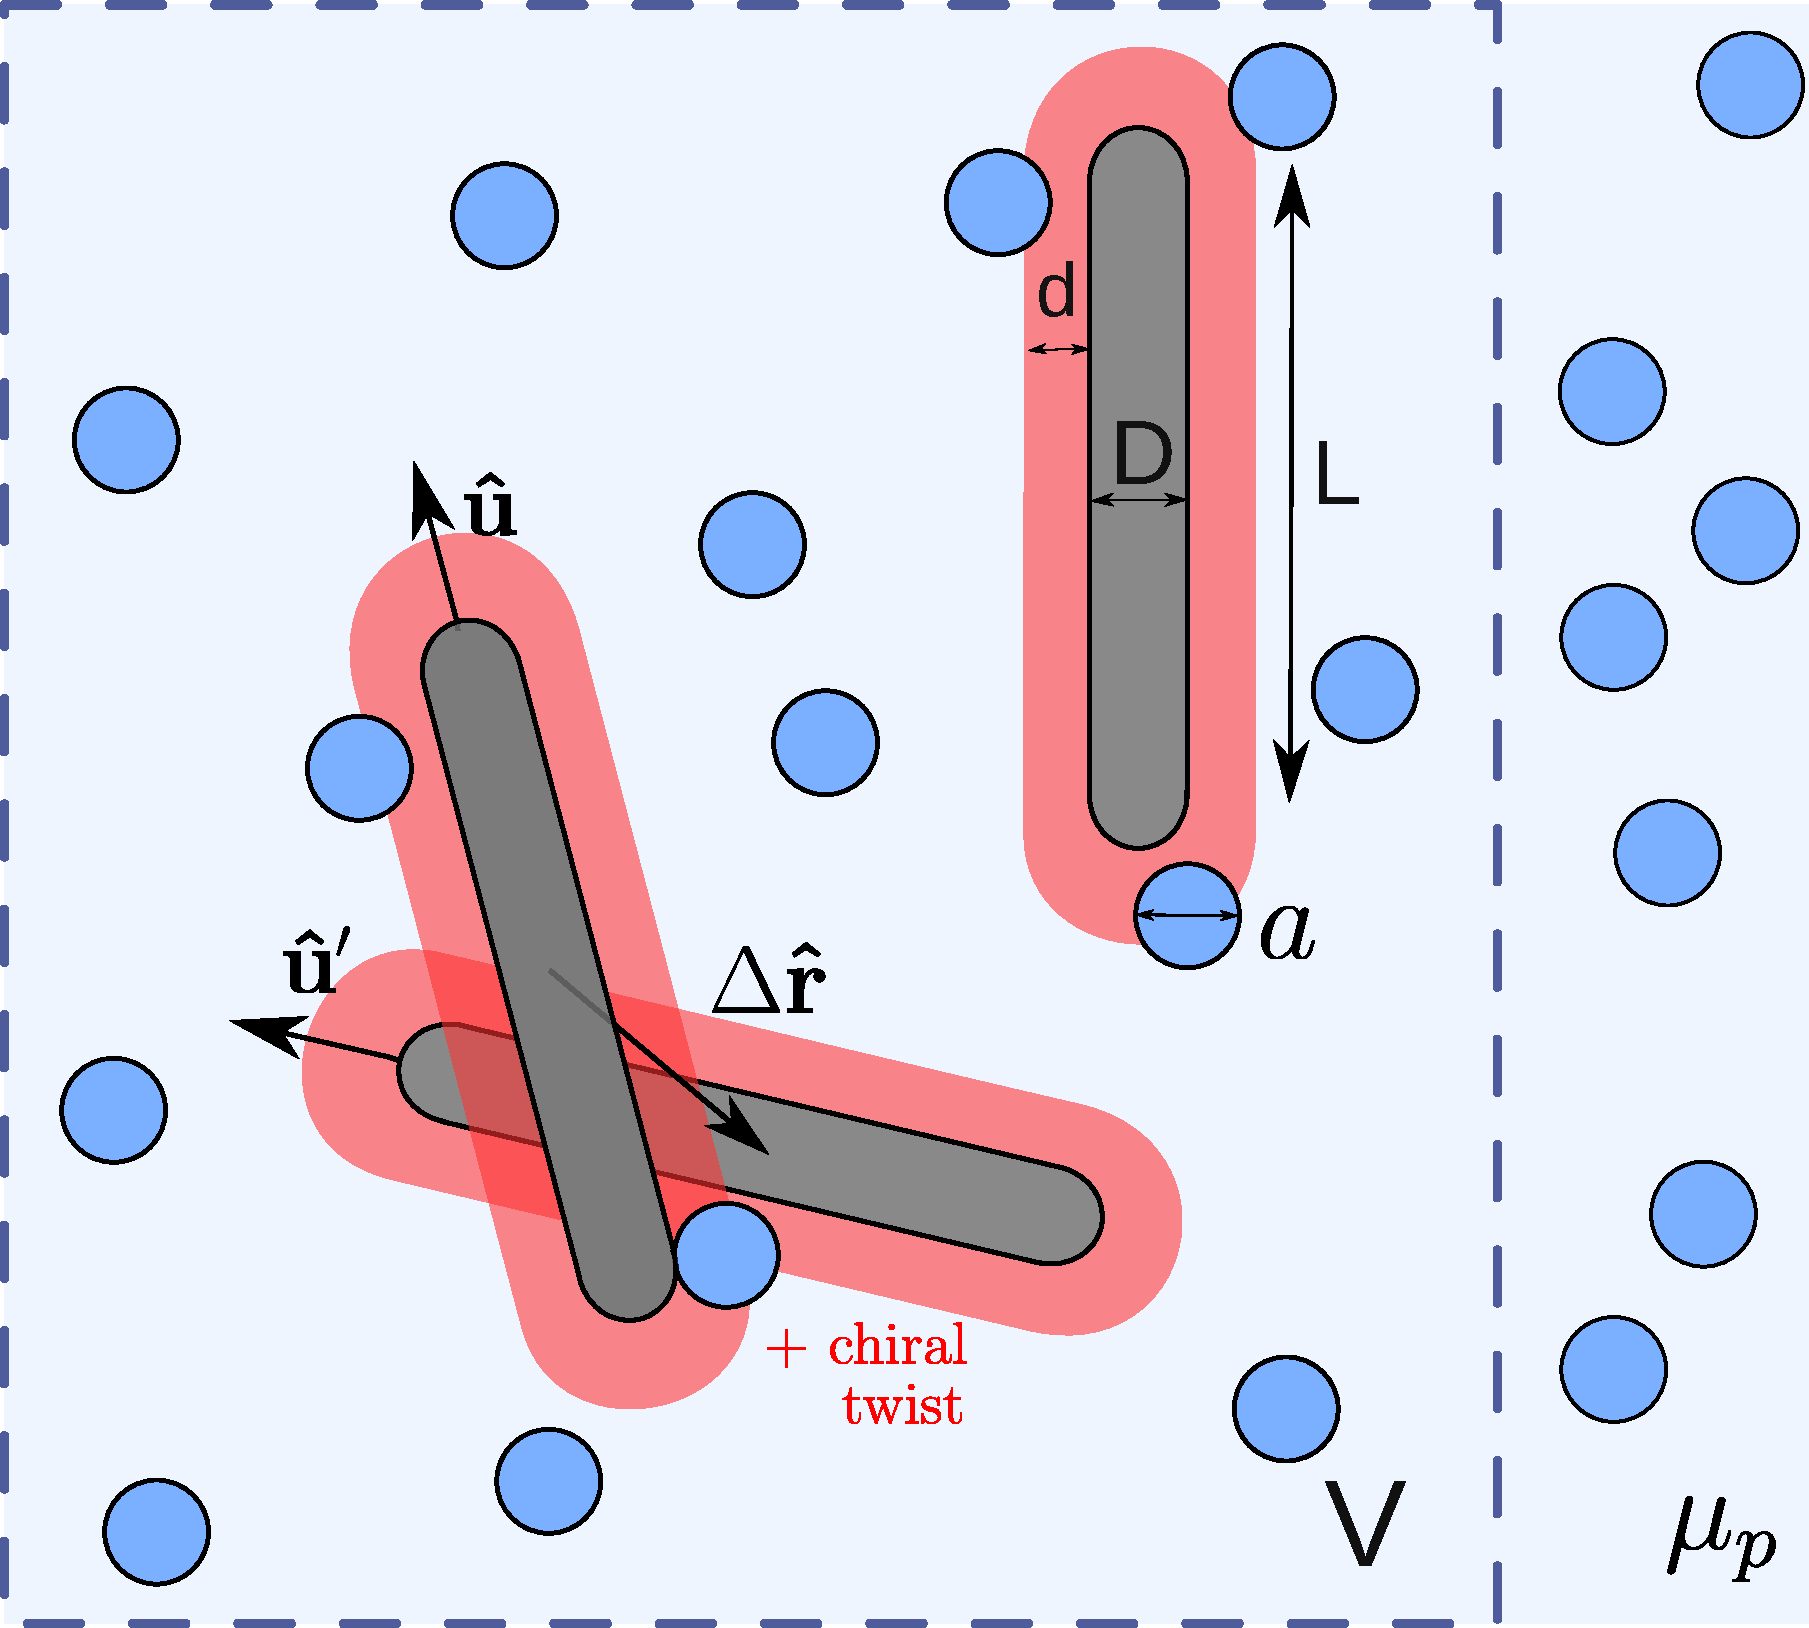
\includegraphics[width = 0.6\columnwidth]{figures/chapter-5/spheromans}
	\caption{ Sketch of the simulation model: hard spherocylinders (grey) mixed non-penetrable polymers (blue) with diameter $\sigma = D$ (as depicted here). Overlap of the cores (grey) gives infinite repulsion while overlapping coronae (blurred zones) favors a twisted pair configuration representing the (chiral) electrostatic forces between {\em fd} rods. The system has a fixed volume $V$ with periodic boundary conditions and connected to a polymer reservoir at constant chemical potential $\mu_p$. }
	\label{sketch}
\end{SCfigure}


\subsection{Chiral interactions}

The pair interaction $U_{r}$ between two spherocylinders with solid angles $\oma$ and $\omb$ and centre-of-mass distance $\Delta \bfr$ follows from a combination of short-range steric forces (treated as strictly hard) and electrostatic forces at larger distance. The  interaction potential between a pair rods depends on centre-of-mass distance vector $\Delta {\bf r}$ and orientation vector $\oma$ of both rods. In our model, the interactions are encapsulated in the following core-shell potential:
\beq
U_{\rm r} (\Delta {\bf r}, \oma, \omb) =
\begin{cases}
\infty & \textrm{if hard cores overlap}\\
U_{\rm twist} & \textrm{otherwise} \\
\end{cases}
\label{urod}
\eeq
The electrostatic interactions between {\em fd} rods gives rise to so-called electrostatic twist which is intimately linked to the chirality surface architecture of {\em fd} virus rods. The chiral  potential is commonly expressed in terms of a pseudoscalar form initially put forward by Goossens \cite{goossens}:
\beq
U_{\rm twist} (\Delta {\bf r}, \oma , \omb )=
-\varepsilon_{c} \left ( \frac{D}{\Delta r} \right )^{7}(\oma \cdot \omb)(\oma \times \omb \cdot \Delta \hat{\bf r})
\label{uchiral}
\eeq
where  $\Delta \hat{\bf r} $ denotes a unit vector for the centre-of-mass distance.
 The sign of $\varepsilon_{c}$ defines the microscopic handedness of the rods. Without loss of generality we take $\varepsilon_{c} > 0$ reflecting the right-handedness of {\em fd} rods. The chiral symmetry of the potential is expressed by the pseudoscalar that imparts a sign change upon  inversion $\Delta \hat{\bf r} \rightarrow - \Delta \hat{\bf r}$. In view of its rapid decay with $\Delta r$ the potential is very short-ranged and the rods need to be very close together in order to feel the chiral twist.

 %For simplicity, we assume that the twisting forces are sufficiently short-ranged (which should be the case at sufficient ionic strength) and do not  continuously vary with the centre-of-mass distance between the spherocylinders, but are only operative if the coronae between the rods overlap (see \fig{sketch}).


\subsection{Estimation of the depletion strength for two parallel spherocylinders}

 The typical attraction energy between two rods due to polymer depletion can be estimated from free-volume theory \cite{LekkerkerkerTuinier2011} and reads:
 \beq
 U_{\rm r,dep} \sim -\Pi_{P} V_{\rm r, ov}
 \eeq
with $ \Pi_{P} = k_{B} T N_{P}/V$ the (van't Hoff) osmotic pressure of the polymer reservoir and $V_{\rm r, ov}$ the overlap volume  of the depletion layers surrounding each rod which depends on the orientation of each rod. In case the rods are perfectly parallel and at hard-core contact we find a simple analytical result. Ignoring  finite rod size effects we have:
\beq
V_{\rm r, ov} = LD^{2} \left [  2 r^{2} \cos^{-1} \left ( \tfrac{1}{2r} \right )  - \tfrac{1}{2} \sqrt{4 r^{2} -1}  \right ]
\eeq
with $r = \tfrac{1}{2}(1 + \tfrac{\sigma}{D})$. Rescaling in terms of the polymer packing fraction in the reservoir we find that the maximum depletion strength per rod pair  reads:
\beq
  U_{\rm r,dep} \sim - k_{B}T \phi_{P}  \frac{L}{D} \left ( \frac{D}{\sigma} \right )^{3} \left [  2 r^{2} \cos^{-1} \left ( \tfrac{1}{2r} \right )  - \tfrac{1}{2} \sqrt{4 r^{2} -1} \right ]
 \eeq
For a typical set-up ($\phi_{P} =3$, $\sigma = 2D$ and $L/D=10$) this gives about 15 $k_{B}T$ \red{Please verify this}.

A key parameter in this system is the relative strength of chiral twist versus depletion attraction. These can be combined into a dimensionless parameter $\chi_{T}$ balancing the energy scales associated with twist and depletion as previously discussed:
\beq
\chi_{T} = \frac{\varepsilon_{c}}{U_{\rm r, dep}} \ll 1
\eeq
so that twist becomes more prevalent for larger $\chi_{T}$. It is important to keep in mind that the typical energy due to chiral twist should be small ($ | \varepsilon_{c} | \ll U_{\rm r,dep} $) in order to ensure that the cohesive forces among the rods residing in a droplet are dominated by polymer depletion, with chiral twist playing only a perturbative role.

\subsection{Semi-grand canonical Monte Carlo simulation}
% TODO: change this section to add Glaser's Algorithm

The simulations are carried out in the semi-grand ensemble, with a fixed number of rods but the polymer content in the system fluctuating against a virtual reservoir consisting of an ideal gas of polymer spheres with a prescribed chemical potential  $\mu_{p}$ which is trivially connected to the polymer packing fraction via:
\beq
\phi_{P} = \frac{\pi D^{3}}{ 6 \Lambda_{p}^{3} } e^{\beta \mu_{P}}
\eeq
where $\Lambda_{P}$ denotes the thermal (de Broglie) wavelength.

\subsubsection{Version I: Explicit depletants}

Each MC cycle consists of $N + N_{P}$ randomly chosen rod translations, rotations, polymer insertions or removals.

\subsubsection{Version II: Implicit depletants}

\red{Here we need to specify Glaser's cluster move optimization algorithm that we used \cite{glaser2015parallel}.}

%\subsection{Rod-wall interactions}

%One possible variation of our model is to confine the rods and polymers in a thin slab of width $h = L$ (see \fig{sketch}). The wall-spherocylinder interactions  are strictly hard, that is, infinite repulsion when the spherocylinder core overlaps with the wall and zero repulsion otherwise. More specifically:
%\beq
%U_{\rm w} (\Delta {\bf r}, \oma) =
%\begin{cases}
%\infty &  | \Delta {\bf r} \cdot {\bf \hat{n}} | < \frac{L}{2}  | \oma \cdot {\bf \hat{n}} | + \tfrac{D}{2} \\
%\infty &   h-  | \Delta {\bf r} \cdot {\bf \hat{n}} | < \frac{L}{2}  | \oma \cdot {\bf \hat{n}} | + \tfrac{D}{2} \\
%0 & \textrm{otherwise}
%\end{cases}
%\label{urodwall}
%\eeq
%with ${\bf \hat{n} }$ denoting the wall normal.

%Polymers are not allowed to overlap with the wall. However, another parameter of the system is the wall depletion range $\sigma_W$ that will take values typically lower than $\sigma$. This strategy is aimed to tune the amount of wetting felt by the tactoids close to the wall, allowing equilibration of partial wetting scenarios. A physical argument for this reduction of the wall depletion range (that in principle would only depend on the size of the depletants), is the variation of the electrostatic forces affecting superficial charges both around the rods and the wall, that may change the effective size of the depletion regions unfavorable for the non-adsorbing polymers.
%The polymers do not have any interaction with the wall, but their centres-of-mass are constrained  to reside within the slab.

\subsection{Simulation methodology} % TODO: change this title??

Monte Carlo simulations are performed for different scenarios conceived from the specifications of the previous sections.

The step size for the spherocylinder translations and rotations are chosen adaptively such as to maintain an average acceptance ratio of about 30 \%. The MC code is optimized using cell-linked list routines that significantly reduce the number of overlap checks between rod-rod and rod-polymer pairs involved in  each MC step. We keep a rectangular box shape with $L_{x} = L_{y}$ and $L_{z} = h = L$ and periodic boundary conditions (PBC) in both lateral directions.

%Depending on the polymer size and concentration the system will either evolve into a liquid drop ("tactoid") or  will retain its crystalline inner structure (expected for `sticky' depletion forces induced by small polymers, $\sigma = D$).
We monitor the total overlap volume of the depletion layers $V_{\rm T, ov}$ and the total twist energy $\mathcal{U}  = \sum_{i}\sum_{j<i}U_{\rm twist}$ to gauge whether the drop has reached its equilibrium state.

We plan to focus on two different systems:

\begin{itemize}
\item  Small polymers with $\sigma = D$ imparting short-ranged attractions. The initial configuration is a square monolayer of perfectly parallel rods ordered into a hexagonal lattice. Without confinement, the cluster will equilibrate into a membrane with  fluid order. In. our simulations we fix the polymer concentrations $\phi_{P}=1$ and $N=2000$. Note that small changes in $\epsilon_{c}$ may have large consequences for the way the droplet expresses chiral twist. At weak twist ($\varepsilon_{c} < ****$), the membrane remains circular in shape with twist showing up at the membrane edges while the membrane center remains largely unperturbed. At strong twist ($\varepsilon > ****$) the membrane may transform into a twisted ribbon. \red{The first indication of such a change of droplet morphology can be observed in \fig{samples} a and c.   Bigger systems ($N=2000$) spontaneously form ribbon-shaped protrusions around a circular central body which resembles the onset of twisted ribbon formation.  }.  Next we introduce confinement and re-assess the droplet shape and internal structure and compare with experimental observations.

\item Large polymers with $\sigma = 2 D$ imparting long-ranged attractions. We start from the same monolayer crystal which will equilibrate into a liquid tactoid in bulk \cite{kuhnhold2022structure}. Gradually increasing the confinement (at $R_{2} > h$ with $R_{2}$ the minor curvature radius of an unconfined tactoid \cite{kuhnhold2022structure})  will lead to squeezed tactoids which  develop a distinct biaxial shape. Introducing twist may lead to further morphological changes. We may correlate droplet size ($N$) with droplet aspect ratio for the strongly confined case compared to the 3D case studied in \cite{kuhnhold2022structure}.

\end{itemize}

%\begin{itemize}
%\item  Small polymers with $\sigma = D$ imparting short-ranged attractions. The initial configuration is a square monolayer of perfectly parallel rods ordered into a hexagonal lattice. Without confinement, the cluster will equilibrate into a membrane with  fluid order. In. our simulations we fix the polymer concentrations $\phi_{P}=1$ and $N=2000$. Note that small changes in $\epsilon_{c}$ may have large consequences for the way the droplet expresses chiral twist. At weak twist ($\varepsilon_{c} < ****$), the membrane remains circular in shape with twist showing up at the membrane edges while the membrane center remains largely unperturbed. At strong twist ($\varepsilon > ****$) the membrane may transform into a twisted ribbon. \red{The first indication of such a change of droplet morphology can be observed in \fig{samples} a and c.   Bigger systems ($N=2000$) spontaneously form ribbon-shaped protrusions around a circular central body which resembles the onset of twisted ribbon formation.  }.  Next we introduce confinement and re-assess the droplet shape and internal structure and compare with experimental observations.
%
%\item Large polymers with $\sigma = 2 D$ imparting long-ranged attractions. We start from the same monolayer crystal which will equilibrate into a liquid tactoid in bulk \cite{kuhnhold2022structure}. Gradually increasing the confinement (at $R_{2} > h$ with $R_{2}$ the minor curvature radius of an unconfined tactoid \cite{kuhnhold2022structure})  will lead to squeezed tactoids which  develop a distinct biaxial shape. Introducing twist may lead to further morphological changes. We may correlate droplet size ($N$) with droplet aspect ratio for the strongly confined case compared to the 3D case studied in \cite{kuhnhold2022structure}.
%
%\end{itemize}



\section{Results}


\begin{figure}
\begin{center}
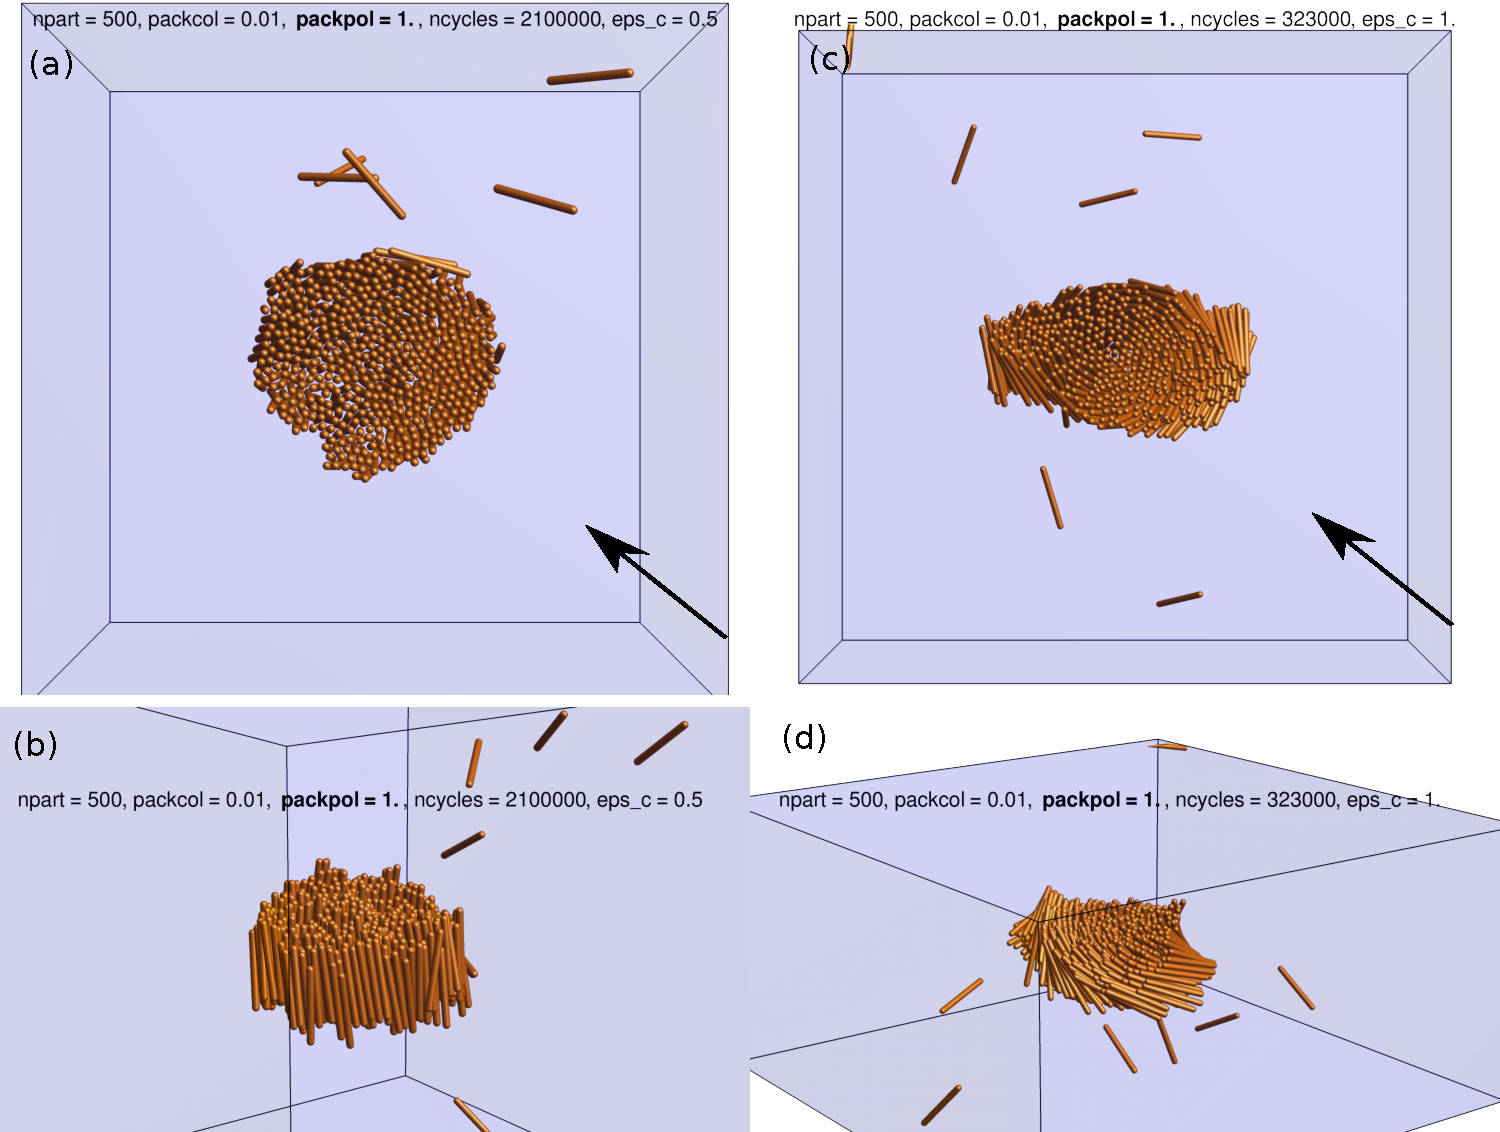
\includegraphics[width= .8\columnwidth]{figures/chapter-5/samples}.
	\caption{Top and front views of membrane-shaped tactoids of chiral rods mixed with non-adsorbing polymer formed in bulk. Color indicates the enclosed angle between each individual rod and membrane normal, from black $\varphi = 0$ to yellow $\varphi = \frac{\pi}{2}$. Shared parameters are $a = 2D$, $\ell = 10$ and $N = 500$. For the cases where vertical fluctuations are (not) allowed, $\phi_P=0.25D^{-3}$ ($\phi_P=0.175D^{-3}$).(a) Low chirality regime. (b) Strong chirality regime showing a cascade of multi-core membranes.}
 \label{multidomain}
\end{center}
\end{figure}


\begin{figure}
\begin{center}
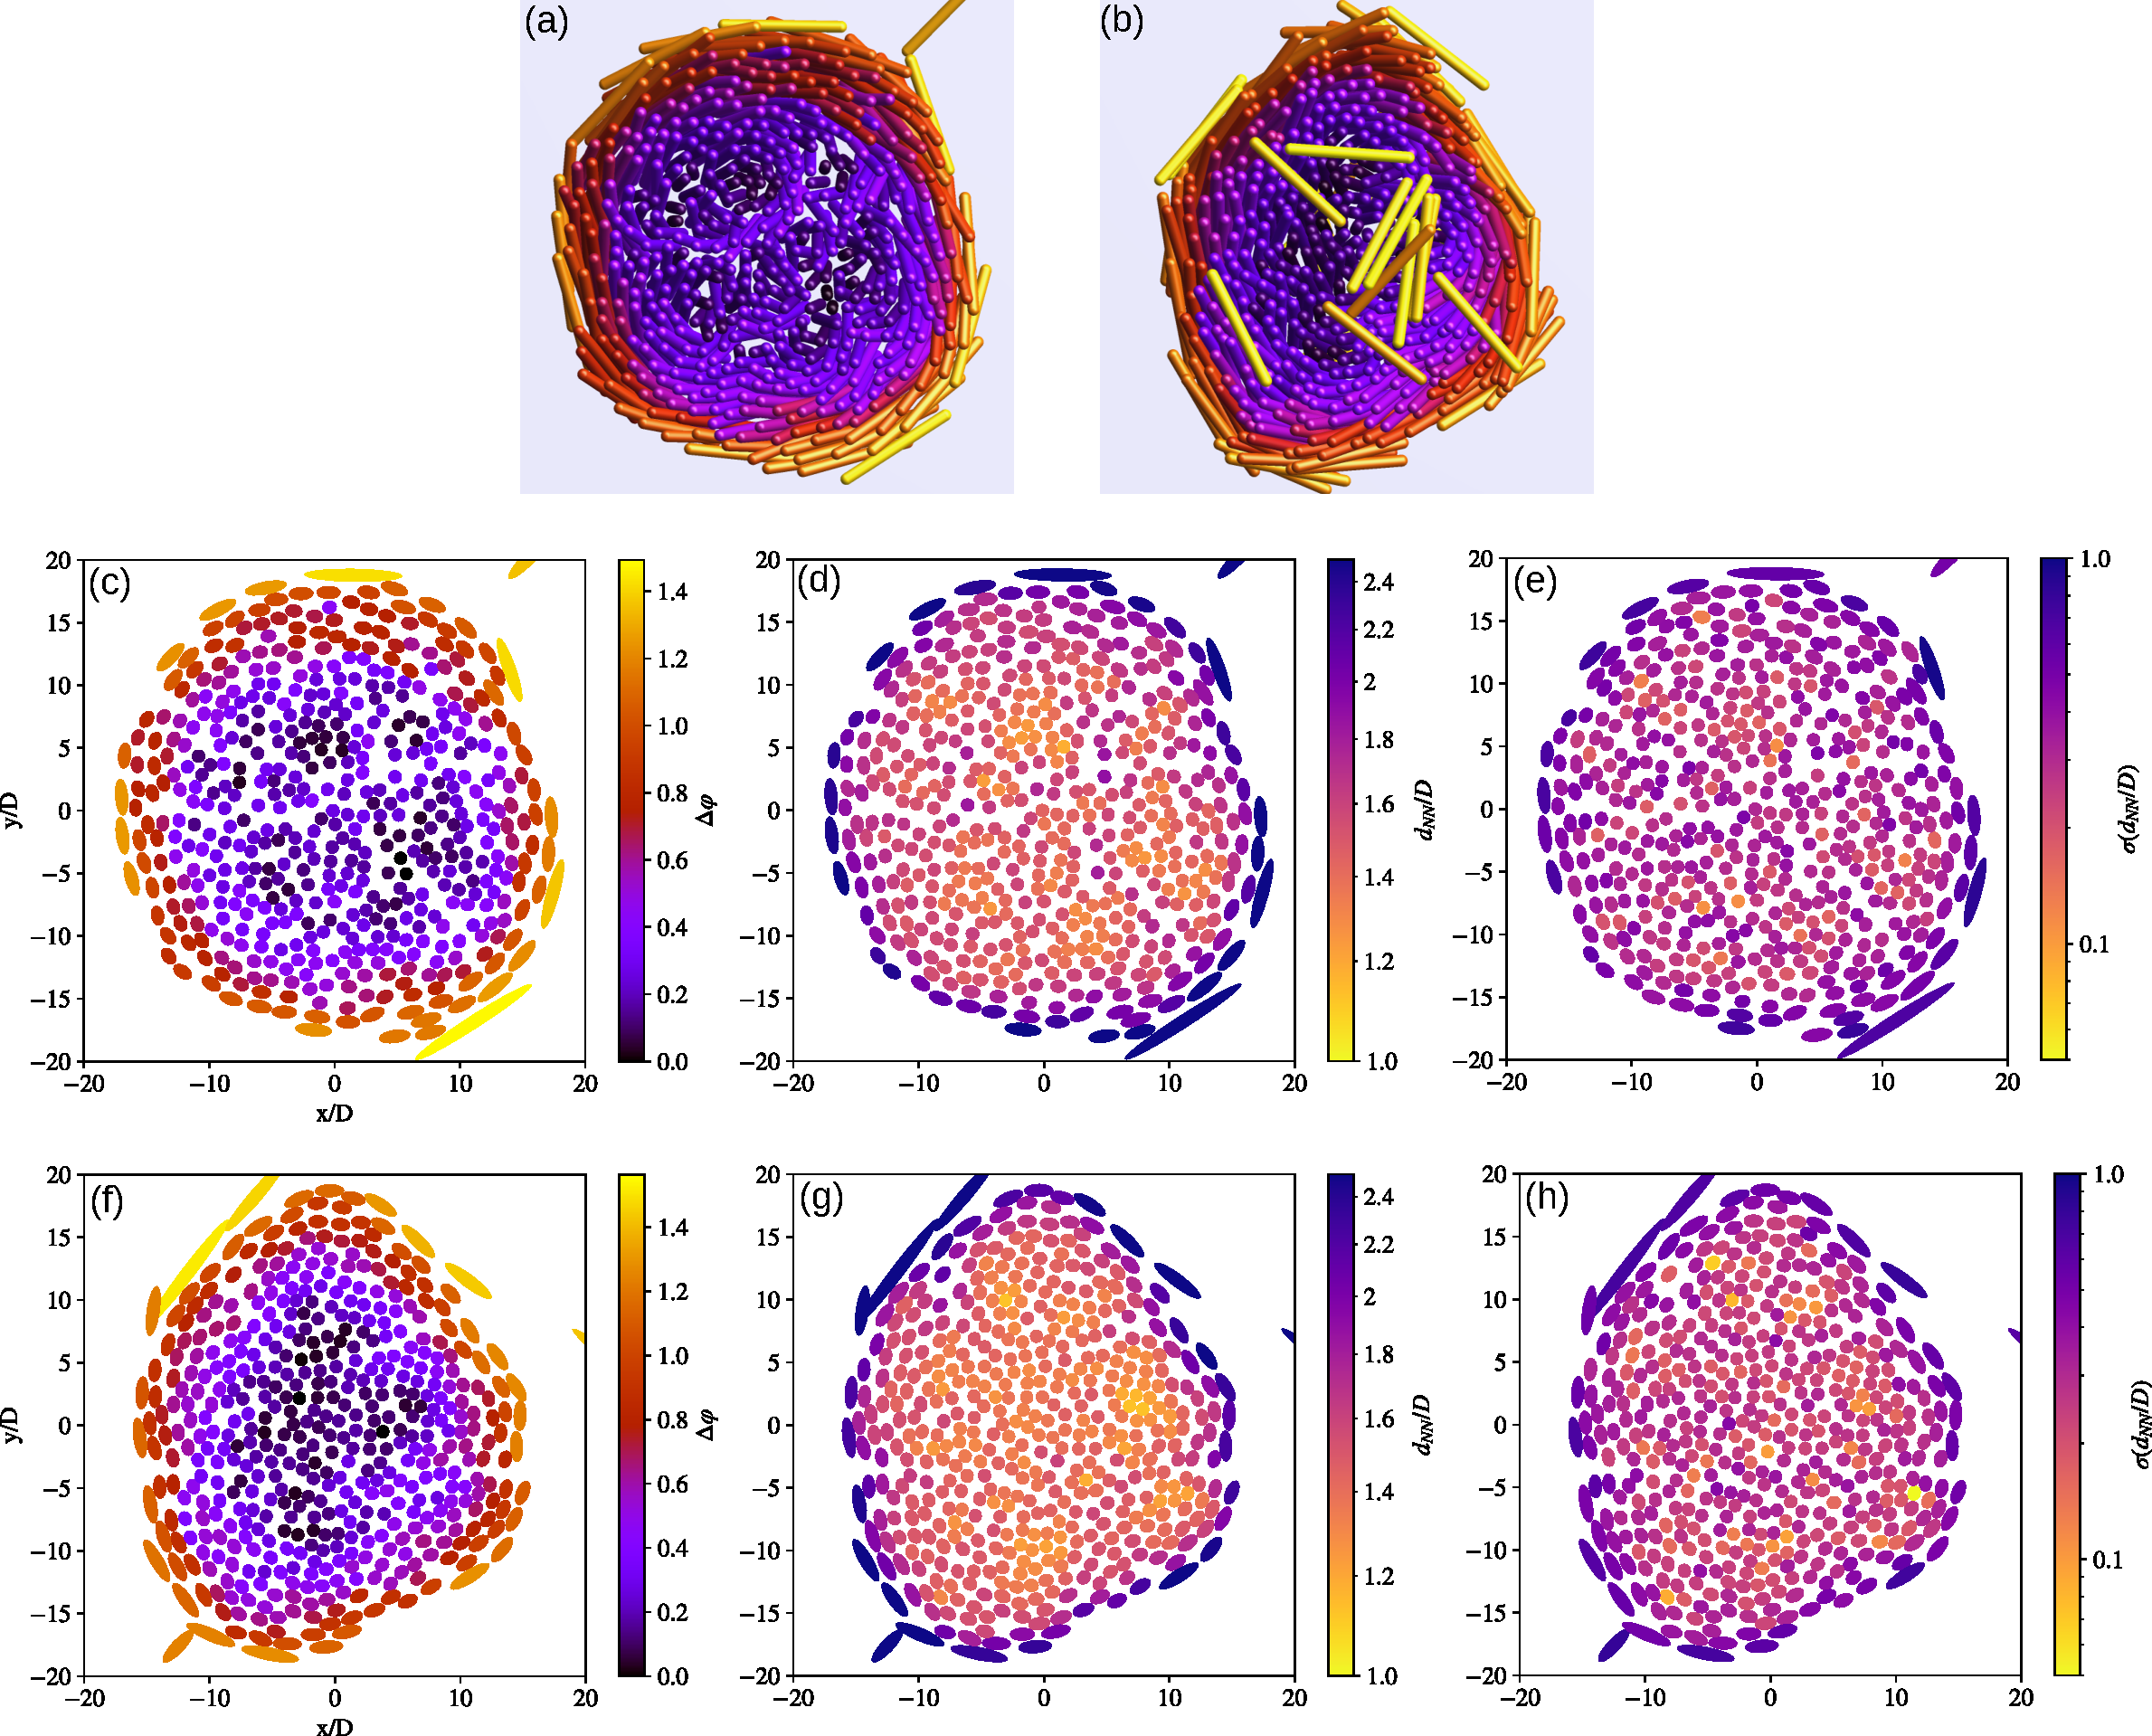
\includegraphics[width= \columnwidth]{figures/chapter-5/crystallinity_11}.
	\caption{ \label{crystal11} Crystallinity of membrane-shaped tactoids of chiral rods mixed with non-adsorbing polymer formed in bulk. Top row: 3D depiction of the system (a) without vertical fluctuations and (b) with vertical fluctuations. Middle and bottom rows: corresponding horizontal sections along the plane generated from a 2D linear regression of the centers of mass of the rods. Upright (untwisted) rods look like disks in this view, while tilted rods appear as ellipses. Color scales indicate: (a)-(c), (f): enclosed angle between the direction of each individual rod and the overall average direction; (d), (g): average distance between each individual rod and its six nearest neighbours; and (e), (h): nearest neighbour distance's standard deviation. Shared parameters are $a = 2D$, $\ell = 10$, $N = 500$ and $\varepsilon_c=11$. For the case where vertical fluctuations are (not) allowed, $\phi_P=0.25D^{-3}$ ($\phi_P=0.175D^{-3}$).}
\end{center}
\end{figure}


\begin{figure}
\begin{center}
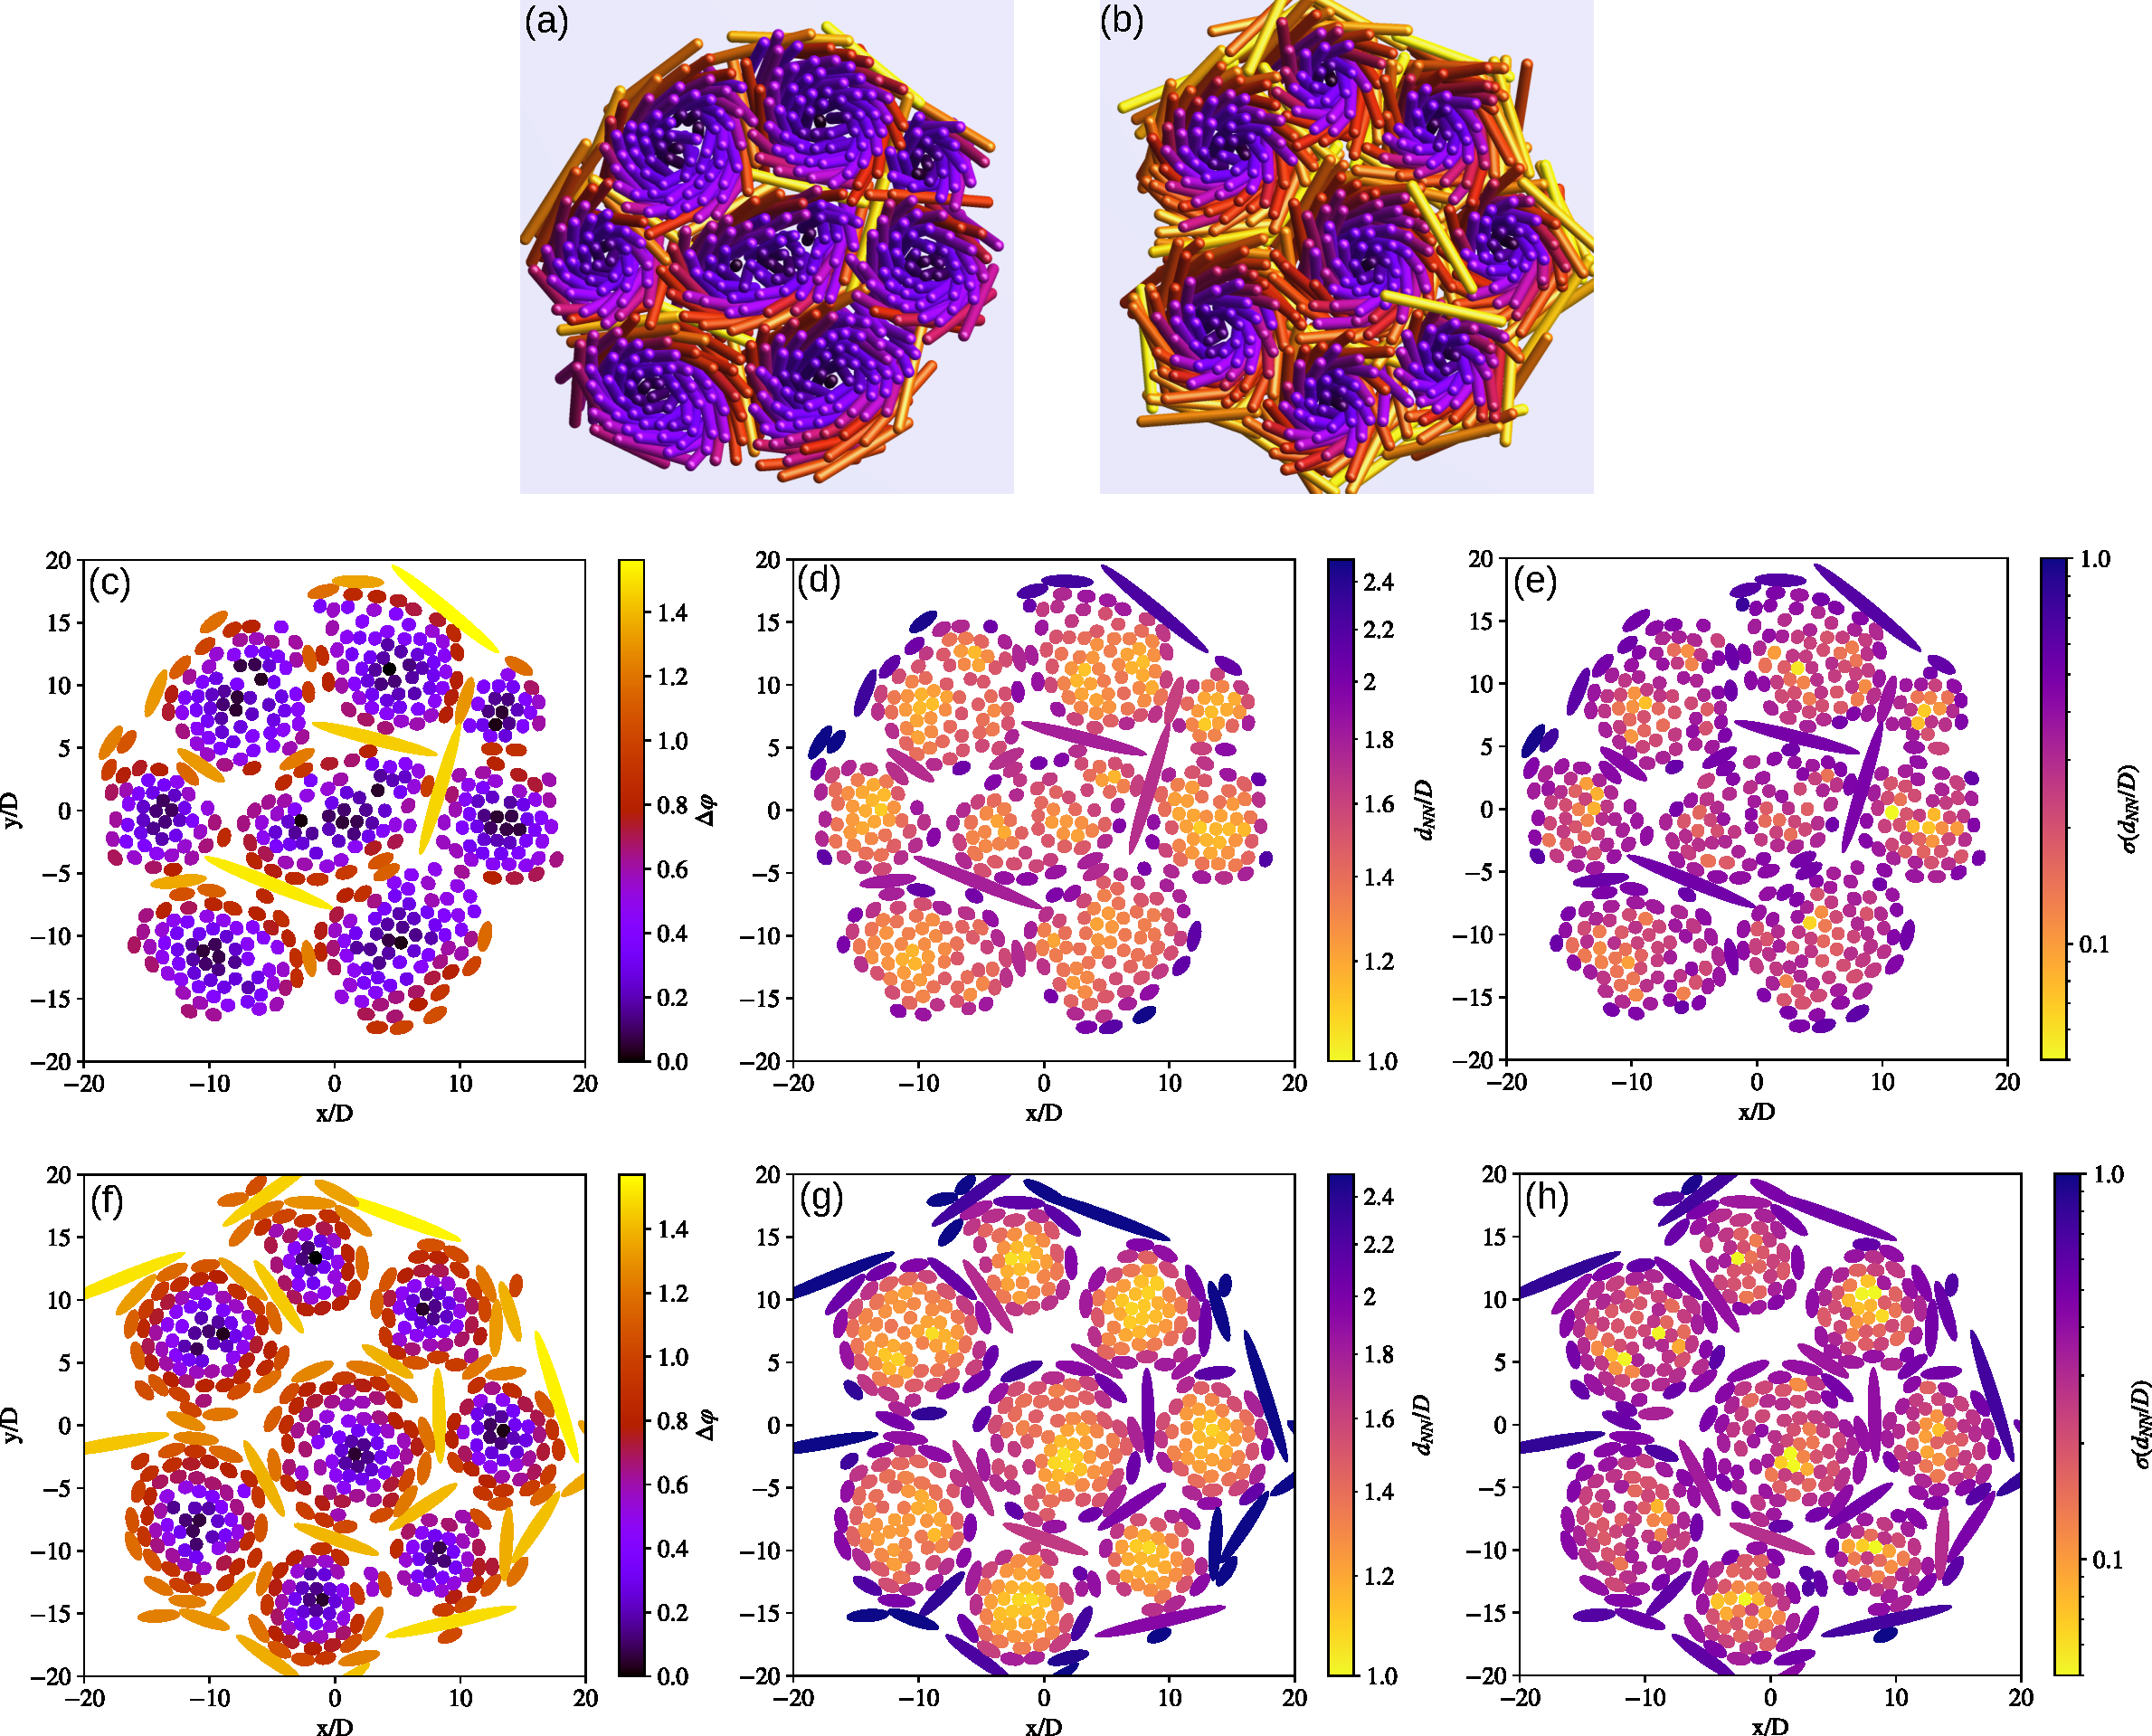
\includegraphics[width= \columnwidth]{figures/chapter-5/crystallinity_16}.
	\caption{ \label{crystal16} Crystallinity of multi-domain membrane-shaped tactoids of strongly chiral rods mixed with non-adsorbing polymer formed in bulk. What is illustrated in this figure is equivalent to \fig{crystal11} except for the chosen chirality regime ($\varepsilon_c=11$ in \fig{crystal11}, $\varepsilon_c=16$ in this figure).}
\end{center}
\end{figure}


\begin{figure}
\begin{center}
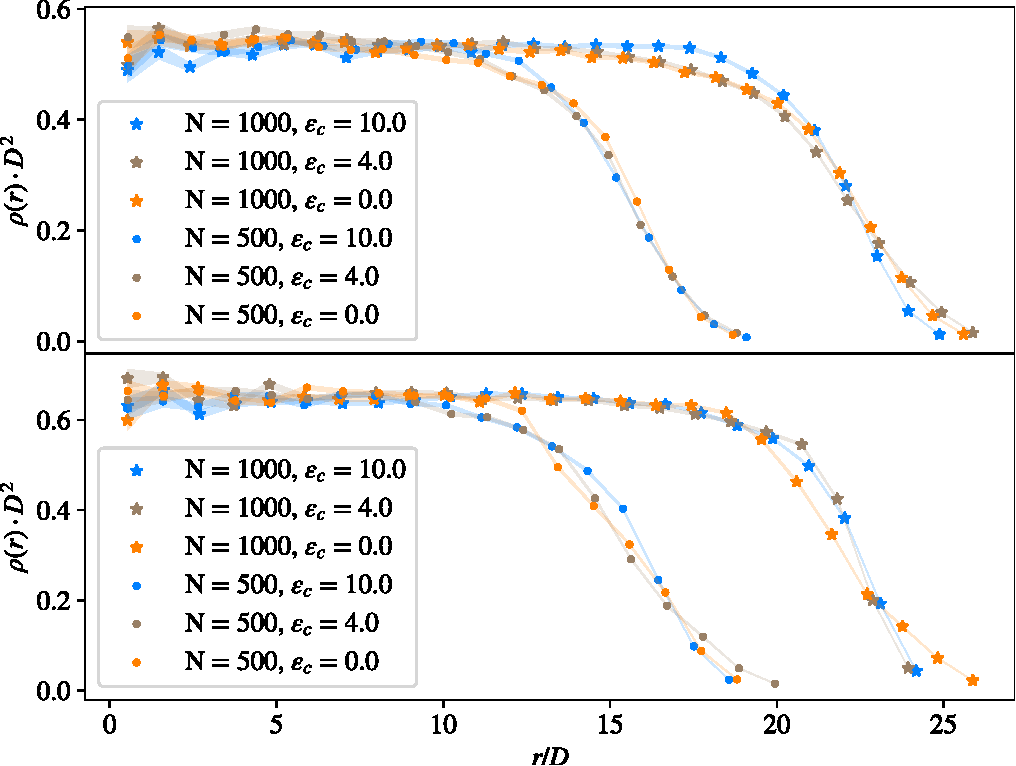
\includegraphics[width= .9\columnwidth]{figures/chapter-5/density}.
	\caption{Rod number density profile of membrane-shaped tactoids of chiral rods mixed with non-adsorbing polymer formed in bulk. Top: without vertical fluctuations. Bottom: with vertical fluctuations. For all cases, $a = 2D$. For the cases where vertical fluctuations are (not) allowed, $\phi_P=0.25D^{-3}$ ($\phi_P=0.175D^{-3}$). } % TODO: explain more.
 \label{density}
\end{center}
\end{figure}


\begin{figure}
\begin{center}
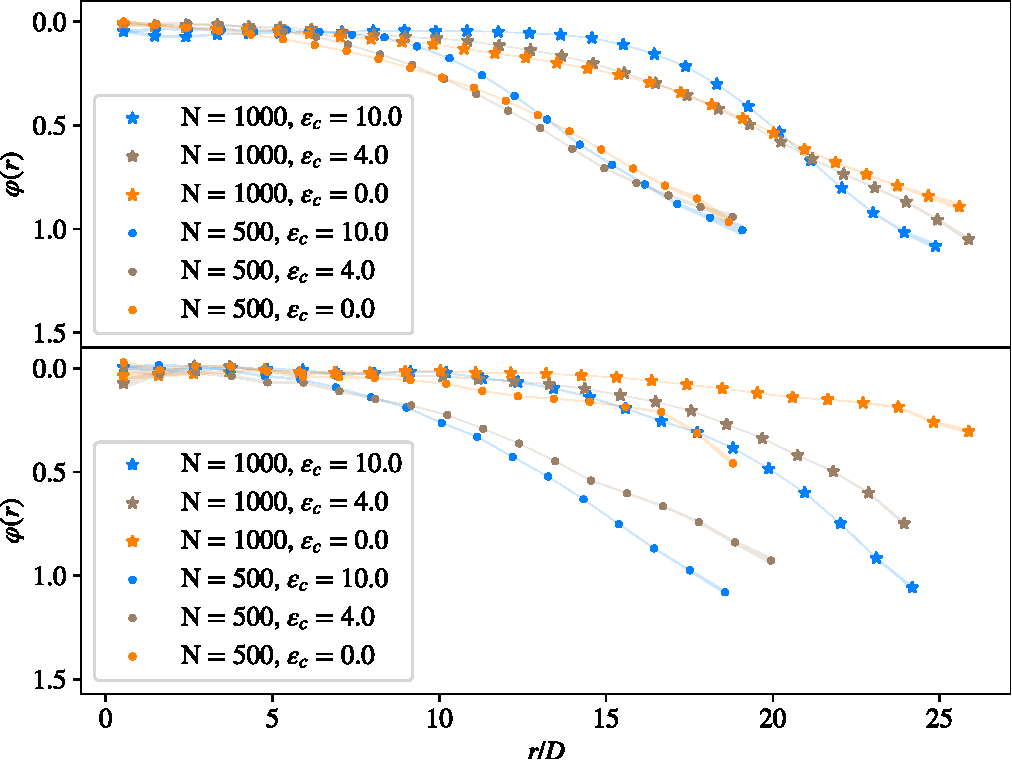
\includegraphics[width= .9\columnwidth]{figures/chapter-5/twistprofile}.
	\caption{Twist angle profile of membrane-shaped tactoids of chiral rods mixed with non-adsorbing polymer formed in bulk. Top: without vertical fluctuations. Bottom: with vertical fluctuations. For all cases, $a = 2D$. For the cases where vertical fluctuations are (not) allowed, $\phi_P=0.25D^{-3}$ ($\phi_P=0.175D^{-3}$). } % TODO: explain more.
 \label{twangle}
\end{center}
\end{figure}


\begin{figure}
\begin{center}
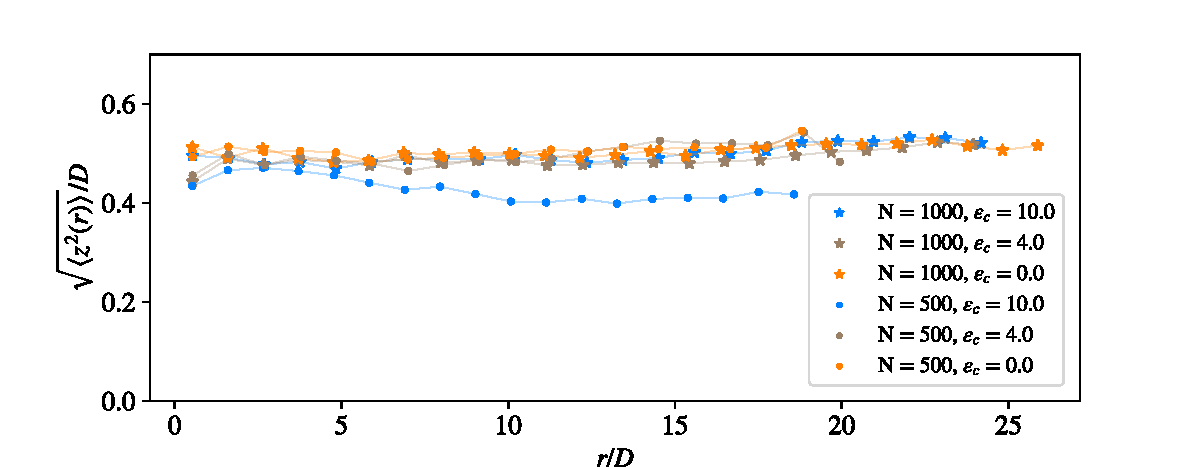
\includegraphics[width= \columnwidth]{figures/chapter-5/zstd}.
	\caption{Vertical fluctuations as a function of the distance to the center of 3D membrane-shaped tactoids of chiral rods mixed with non-adsorbing polymer formed in bulk, $a = 2D$, $\phi_P=0.25D^{-3}$. } % TODO: explain more.
\end{center}
\end{figure}





\section{Theory for twisted membranes}




\begin{SCfigure}
\includegraphics[width= 0.4 \columnwidth]{figures/chapter-5/membrane_sketch}.
\caption{ \label{memsnap} Schematic structure (top and front view) of a twisted smectic membrane of radius $R_{m}$ composed of strongly chiral spherocylinders with aspect ratio $\ell = 10$ mixed with non-adsorbing polymers (not shown) providing strong side-to-side depletion attraction between the rods.  The top graph depict the top view, the lower one a side view of the membrane. The director twist, expressed by the twist angle $\varphi$, is zero at  the membrane  core $\bn _{\rm core} = \bz$ and increases concentrically with radius $R$.}
\end{SCfigure}




 To complement our simulations results we now develop a theory for twisted membranes by focussing on two distinct morphologies that have been observed in experiment, namely half-skyrmion-type membranes and twisted ribbons. In both cases, the twisting of the rods occurs in both principal directions of the membrane (double twist), whereas the cholesteric phase exhibits unidirectional twist. Somewhat confusingly, double twist may also refer to the case of {\em chiral ribbons} in which the membrane itself is wrapped 
in a helical fashion thus exhibiting non-zero mean curvature \cite{green1936equilibrium,chopin2016roadmap}. Although these chiral ribbons have also been observed in {\em fd} polymer mixtures under cetain conditions \cite{Gibaud2012} but we will not consider this particular case in our model.
 
 
 Let us begin by recalling the well-known Frank-Oseen elastic energy of the general case of a bulk chiral liquid crystal for and arbitrary nematic director field $\bn$ in three spatial dimensions:
\begin{align} 
F = & \frac{1}{2} \int d \bfr \left [ K_{1} (\nabla \cdot \bn)^{2}  + K_{2} (\bn \cdot \nabla \times \bn + q_{0})^{2}  +   K_{3} (\bn \times \nabla \times \bn)^{2} \right ]  
\end{align}
with $K_{1}$, $K_{2}$ and $K_{3}$ respectively denoting the splay, twist and bend elastic moduli.   The inverse  pitch  $q_{0}$ quantifies the chiral strength of the particles in the liquid crystal. 


 For the specific case of a cylindrically symmetric, twisted membrane depicted in\fig{memsnap}
  with radius $R_{m}$ we may invoke a cylindrical geometry  with radial coordinate $0<R< R_{m}$ and angle $\alpha$.  Deformations from a uniform director field in which case $\bn = \bz$ are assumed to be concentric and can be described as:
 \beq
 \bn = \cos \psi (R) \cos  \varphi(R) \bz + \cos \psi (R) \sin \varphi(R) \bal + \sin \psi(R) \bars
 \label{tilt}
 \eeq
in terms of a twist angle  $ \varphi $ denoting a twist deflection of the rods with respect to the membrane normal and $\psi$ a splay deformation along the membrane radial vector (see \fig{memsnap}).   We the local rod density within the membrane to be uniform so that the one-body density reads $\rho(R, \bw)  = \rho_{0}f(R,  \bw)$, in terms of the rod number density $\rho_{0}$ denoting the number of rods per area unit, and a three-dimensional rod unit vector $\bw$ distributed along the local director obeying an a priori unknown distribution $f$. The twist-bend elastic free energy  takes the following form \cite{barry_jpcb2009,wensink2018elastic}:
\begin{align}
 F_{el}  &= \int  d \brr \left [ K_{2} \left ( \partial_{R} \varphi + \frac{\sin 2 \varphi}{2R} + q_{0} \right )^{2}  + K_{3}\frac{ ( \sin \varphi )^{4}}{R^{2}} \right   ]
\label{fmem}
\end{align}
with $\int d {\bf R} = 2 \pi \int_{0}^{R_{m}} R dR $ in circular coordinates for a membrane with radius $R_{m}$.
 The  elastic moduli for the membrane are distinctly different from those of a ulk liquid crystal and will be specified in the next section. We remark that these elastic moduli are strictly 2D quantities with dimension energy.  


In an earlier version of our theory \cite{wensink2018elastic} the effect of depletion attraction due to the non-adsorbing polymer can be described in terms of a simple free energy 
\beq
F_{dep}  \sim U_{0} \int d \brr  (\sin \varphi )^{2}  + {\rm cst}
\eeq
where $U_{0}$ is a tilt energy density (per unit area) related to the osmotic pressure of the polymer reservoir and polymer radius of gyration. The simple sine squared contribution is chosen here for simplicity and is in line with de Gennes' original treatment of twist expulsion towards the edges or around defects of smectic layers in analogy with superconductors \cite{gennes-prost, barry_jpcb2009}. It captures the basic trend that the local director tilting away from the membrane normal compromises the free volume experienced by the non-adsorbing polymer  thereby inducing a free energy penalty. In our theory, out-of-plane fluctuations of the rod centre-of-mass away from the 2D plane are not included, but this can be done so on a simple mean-field level \cite{kang_sm2016}.
Ignoring the curvature terms  $R \rightarrow \infty $ and considering a smectic layer on an infinite half-plane enables an analytical minimisation of the free energy in terms of the twist penetration depth $\lambda_{t}  =  \sqrt{K_{2}/a} $ \cite{gennes-prost,barry_jpcb2009}. For the circular membrane, a simple simulated-annealing Monte Carlo algorithm can be employed to minimise the free energy with respect to the twist angle $\varphi(R)$ for any given triplet of length scales, namely the bulk cholesteric pitch $q_{0}^{-1} $, twist penetration depth $\lambda_{t} $ and membrane radius $R_{m}$. With the twist elastic modulus and chiral amplitude being microscopically defined \eq{kexp} a simple one-parameter fitting procedure can be used to determine the depletion strength $a$ and the twist penetration depth $\lambda_{t}$. 



 The main features we established from the numerical results \cite{wensink2018elastic} are the following:  (i) the twisting becomes more pronounced toward the membrane edge when the twist penetration depth becomes shorter, as expected,  but also when membrane size grows larger. (ii) Increasing the pitch $q_{0}$  enhances the maximum twist angle while keeping the overall shape of the twist angle profile largely unchanged. (iii) The local splay angle remains negligibly small  across the membrane so that the omission of splay effects seems fully justified.




\subsection{Scaling results for the elastic moduli for a fluid membrane}

Using second-virial theory combined with a Gaussian approximation for the orientation probability of the rods within the membrane one can estimate the leading-order contributions of the torque-field, splay, twist and bend elastic constants of a membrane, respectively:
\begin{align}
  K_{1}   & \sim  \frac{17 \rho_{0} \ell^{2}}{24} = \frac{17}{2} K_{2}   \nonumber \\ 
 K_{2}  & \sim  \frac{\rho_{0} \ell^{2}}{12}   \nonumber \\ 
 K_{3} &\sim  \frac{1}{4} K_{2}
  \label{kexp}
\end{align}
Note that the membrane moduli have unity ${\rm N \cdot m}$ (the 3D moduli would be expressed in Newtons) and $\rho_{0} = ND^{2}/A$ refers to planar density of rods with diameter $D$, aspect ratio $\ell = L/D$ and membrane area $A$. The results suggest that the moduli of rodlike particle confined to a membrane are quite different from those of of 3D bulk nematic fluid, at least for strongly elaongated rods experiencing strong nematic order.  In the limit of asymptotic alignment, the splay-to-twist ratio of a bulk fluid  \cite{odijkelastic}  was predicted to scale as $K_{1}/K_{2} \sim 3 $ whereas a much higher ratio $K_{1}/K_{2} \sim 17/2$ is found for the membrane. The bend-to-twist ratio for a hard rod nematic fluid was found to be proportional to the degree of nematic alignment $K_{3}/K_{2} \sim \sigma \gg 1$ \cite{odijkelastic} where $\sigma$ is steered by the rod concentration.  The curvature-to-twist elasticity of a membrane turns out to be smaller than unity $K_{3}/K_{2} \sim 1/4$ and independent of the rod concentration.  In other words, rods confined to a membrane experience a much stronger resistance to splay fluctuations whereas  bend fluctuations are far less penalised compared to a 3D nematic fluid.  Since the splay modulus is about an order of magnitude larger than the twist elasticity, we expect director deformations whereby rods tilt along the radial vector of the membrane to be of marginal importance and  will be ignored.  





\subsection{Chiral twist }

The pitch $q_{0}$ of a twisted membrane can be estimated by considering a weakly chiral pair potential $U_{c}$ described by some arbitrary but short-ranged spatial decay function $g(r)$ describing the range over which chiral forces interact and chiral amplitude $\varepsilon_{c} $ much smaller than the thermal energy. This potential takes the following generic form \cite{goossens1971}:
\beq
U_{c} \sim  \varepsilon_{c} g( r)(\bwa \times \bwb \cdot   \bx) (\bwa \cdot \bwb)
\label{uchi}
\eeq
From this, we may compute the so-called torque-field constant exerted by the chiral potential \cite{wensink2018elastic}:
\beq
K_{t}   \sim -\rho_{0}^{2}  \bar{\varepsilon}_{c} 
\eeq
in terms of an integrated chiral amplitude  $\bar{\varepsilon}_{c}$ which is  {\em different} from that of a  3D cholesteric system as it implicitly encodes the geometric confinement given that $\bdr$ is a 2D vector:
\beq
 \bar{\varepsilon}_{c}  =  \varepsilon_{c} \int d \bdr | \bdr \cdot \bx |    g( r)
 \eeq
 which has units energy times volume ($k_{B}T \times D^{3}$). The chiral potential drives the twisting of the membrane and $K_{t}$  provides an explicit link between the effective torque-field and the range and amplitude  of the chiral pair potential between a pair of  rods. We remark that the above mean-field treatment will be less adequate for strongly chiral amplitudes $\varepsilon_{c} \gg k_{B}T$. A common choice for $g(r)$ is a short-ranged power law $g(r) = 1/r^{7}$ but  long-ranged forms such as a square-well (SW) potential could be conceivable as well \cite{wensinkjackson}. Taking the power law featuring in \eq{uchiral} we obtain $\bar{\varepsilon}_{c} = \varepsilon_{c} D^{3}$.  From this we find a {\em microscopic} expression for the typical equilibrium  pitch of the membrane $q_{0} = K_{t}/K_{2}$ that further depends on the in-plane rod density $\rho_{0}$ and rod aspect ratio $\ell = L/D$:
 \beq
 q_{0} \sim \frac{12 \rho_{0} \bar{\varepsilon_{c}}}{ \ell^{2}}
 \label{qzero}
 \eeq
 While for the single-twisted cholesteric phase the twist angle increases linearly  $\varphi(z) = q_{0} z$ at each position $z$ along the helix axis, the angle will be strongly non-linear with radius $R$ in case of the twisted membrane, in particular if the twist penetration length $\lambda_{t}$ is small \cite{wensink2018elastic}.   
 


\subsection{Effect of depletants and twist penetration length}

Kang et al. \cite{kang_sm2016} have proposed a more sophisticated expression for the effect of the depletion attraction on the twist angle via the local membrane height $h = (L/2) \cos \varphi$: 
\begin{align}
F_{dep}  \sim & 2 n_{p} a k_{B}T \left [ \int  d {\bf R} \sqrt{ 1 + (\nabla h)^{2} } + \oint d {\bf l} h \right ]
\label{fdep1}
\end{align}
with $n_{p}$ the polymer reservoir pressure and $a$ the polymer radius of gyration. The last contribution is identified a line tension generated by depletion forces between rods. Combining this with the elastic part of the 
\eq{fmem} we find the following free energy for a membrane with radius $R_{m}$:
\begin{align}
\frac{ F}{K_{2}}  &\sim \int  d \brr   \left [  \left ( \partial_{R} \varphi + \frac{\sin 2 \varphi}{2R} + q_{0} \right )^{2}  + \frac{K_{3}}{K_{2}}\frac{ ( \sin \varphi )^{4}}{R^{2}} \right . \nonumber \\ 
& \left .  + \lambda_{t}^{-2}    \sqrt{ 1 + (\partial_{R} h)^{2} }   \right ]  + 2 \pi  \lambda_{t}^{-2} R_{m} h(R_{m})
\label{fmem1}
\end{align}
with $\int d {\bf R} = 2 \pi \int_{0}^{R_{m}} R dR $ in circular coordinates. The line tension contribution drops with increasing twist at the edges and  becomes zero if the rods are twisted perpendicular to the membrane normal $\varphi(R_{m}) = \pi/2$. 
The twist penetration length is given by $\lambda_{t} = \sqrt{K_{2}/2  n_{p} a k_{B}T}$ which, using \eq{kexp} leads to a compact expression depending on quantities known from experiment such as the in-plane rod density (assumed uniform across the membrane), rod-polymer size ratio $D/a$, rod aspect ratio $\ell$ and the reservoir polymer concentration $n_{p}$: 
\beq
\frac{\lambda_{t}}{D} = \sqrt{\frac{\rho_{0} \ell^{2} }{24  (n_{p} a^{3}) (D/a)^{2} }}
\eeq
Taking typical numbers from our simulation ($\ell \sim 10$, $\rho_{0} \sim 0.5$, $D/a=2$ and $n_{p}a^{3} \sim 0.2$) we find that that the twist penetration length is only a few times the rod diameter, i.e. $\lambda_{t} \sim 2 D$. This is broadly in line with the twist angle profiles  in \fig{twangle} where the twist expulsion at the edge was found to extend over a typical distance  of about $\sim 5D$.  
For {\em fd} rods a much larger value is found primarily because they are longer than our rods ($\ell \sim 130$). The predicted value $\lambda_{t} \sim 20 D$ is roughly line with the experimentally measured value of about half a rod length   depending on the polymer concentration that was used to stabilize the membranes \cite{barry_jpcb2009}.

In Ref. \cite{kuhnhold2022colloidal} a simple trial form was used to fit the simulation data:
\beq
\varphi(R) = \varphi_{0} \left ( \frac{R}{R_{m}} \right )^{\alpha} 
\eeq
with $\varphi_{0}$ the twist angle at the membrane edge and $\alpha $ a variational parameter governing the degree of twist near the edge.  It is tempting to insert the trial form into the free energy \eq{fmem1} and seek an algebraic minimization route through the variational parameters $\varphi_{0}$ and $\alpha$.   However, such an approach turns out to be too unfeasible because the free energy is strongly non-linear in $\varphi$.  As in Ref. \cite{wensink2018elastic} we therefore employ a simulated-annealing Monte Carlo algorithm to obtain the angular profile as a function of the distance from the membrane core. 

\section{Starfish instability and twisted ribbon}


\begin{figure}
\begin{center}
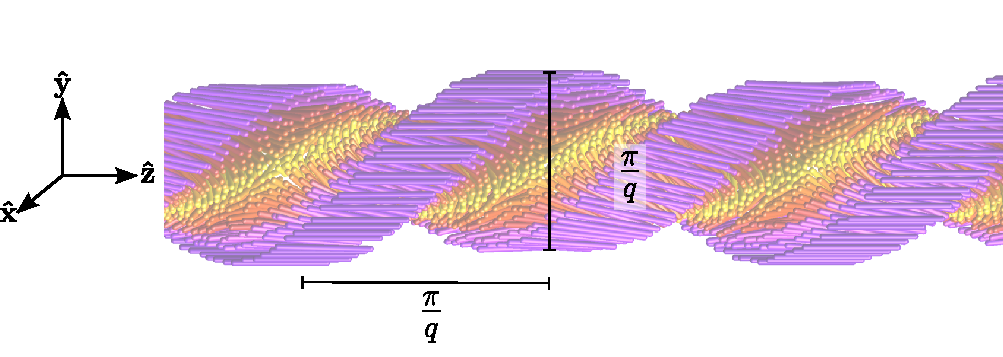
\includegraphics[width= \columnwidth]{figures/chapter-5/ribbon_sketch}.
\caption{ \label{ribsnap} Schematic structure of of twisted ribbon of width $s_y=2\ell$ composed of strongly chiral spherocylinders with aspect ratio $\ell = 15$ mixed with non-adsorbing polymers (not shown) providing strong depletion attraction between the rods. The rods are color coded by orientation. The typical  ribbon dimensions are indicated by the pitch $q$ with $\pi/q$ corresponding to a half pitch length.  }
\end{center}
\end{figure}

At elevated chiral strength the circular membranes are known to transition into twisted ribbons \cite{Gibaud2012}. These were identified as quasi-1D twisted protrusions growing out of the perimeter of the membrane, through a mechanism termed `starfish' instability.


Lowering the temperature strengthens the chiral forces between the rods, which raises the free energy of the interior untwisted rods while lowering the free energy of edge-bound twisted rods. This enables chiral control of edge line tension which, when the edge tension approaches zero,  leads to spontaneously transitions of the membrane into an array of 1D twisted ribbons, called a ‘‘starfish’’ \cite{Gibaud2012}. A phenomenological model aimed at capturing the onset of the surface-driven instability was presented in Ref. \cite{kang_sm2016}. So far, no minimalist theory along the spirit of the one discussed for the membrane has been contemplated for the ribbon whose intricately twisted structure is  depicted in \fig{ribsnap} based on a nematic  director parameterization we are about to present.  While the membrane exhibits double twist in a circularly symmetric fashion, the rods within the ribbon are twisted in two mutually perpendicular directions along the short and long axes of the ribbon.  Then, the director field of a twisted ribbon may be constructed from a combination of two rotation matrices, each corresponding to a twist along mutually perpendicular Cartesian axes. Without loss of generality we fix the director field of the untwisted ribbon along the $x$-axis of the frame $\bn_{0}=(1,0,0)$ so that the director field of the ribbon reads:
\beq
\bn_{r}[ \Phi, \chi] = \mathcal{R}_{xz} [\Phi]\cdot \mathcal{R}_{xy}[\chi] \cdot \bn_{0}
\label{nrib}
\eeq
in terms of the rotation matrices
 \beq
 \mathcal{R}_{xz} [ \Phi]   =
  \begin{bmatrix}
     \cos \Phi(y) & 0 & \sin \Phi(y)  \\
    0 & 1 & 0  \\
    -\sin \Phi(y) &  0 & \cos \Phi(y)  \\
      \end{bmatrix}  \nonumber
      \label{rxz}
 \eeq
and
 \beq
 \mathcal{R}_{xy} [ \chi]   =
  \begin{bmatrix}
     \cos \chi(z) &  \sin \chi(z) & 0  \\
    -\sin \chi(z) &   \cos \chi(z) & 0 \\
      0 & 0 & 1  \\
      \end{bmatrix}  \nonumber
      \label{rxy}
 \eeq
Here, $\Phi$ and $\chi$ denote  two  angles describing the twist along the short and long (ribbon) axes that we parameterize via the coordinates $-s_{y}/2 < y < s_{y}/2$ and $-s_{z}/2< z <s_{z}/2$, respectively. The ribbon area $A = s_{y}s_{z}$ is conserved. We further define the local thickness of the ribbon:
\begin{align}
h = \frac{L}{2}   | \bn_{0} \cdot \bn |  =\frac{L}{2} |\cos \chi(y) \cos \Phi(y)| 
\end{align}
We now simplify matters by assuming linear twist in both directions so that $\chi = qz$ and $\Phi = qy$ where $q$ denotes the principal pitch of the ribbon quantifying the degree of twist along the long and short ribbon axes. We remark that the  ribbon pitch is likely to be different from the value $q_{0}$ that we defined in \eq{qzero} which quantifies the chiral strength between the rods. Henceforth, we will use the ribbon width as our length unit and render all pitches dimensionless via $q \rightarrow q s_{y}$. We assume the ribbon to be long enough so we can ignore surface effects imparted by the short edge of the ribbon. Using the parameterization of the director \eq{nrib} we find that the   contributions corresponding to bend, splay and twist elasticity {\em per unit ribbon length}  reads:
\begin{align}
F_{bend} &=\frac{K_{3}}{16} \left [ 3 q^{2} - q \sin q (\cos q -2)\right ]  \nonumber \\ 
F_{splay} &=  
\frac{K_{1}}{8}  (q^{2}  - q \sin q )  \nonumber \\ 
F_{twist} &=  \frac{K_{2} }{16  }  \left [ 8 q_{0}(q_{0} -q -\sin q)  + q\sin q ( \cos
   q +4) + 7 q^{2}\right ]
\end{align}
Note that the bulk elastic energies   are all {\em even} functions of the pitch $q$, expect the first term in the twist contribution which encodes chirality and vanishes for achiral rods ($q_{0} =0$). 
 We must also consider the effect of saddle-splay, which is nonzero due to the curvature of the ribbon (it does not play a role for the flat membranes). It can be defined in terms of the following bulk contribution to the Frank elastic energy: 
\beq
F_{saddle} = -\frac{K_{24}}{2} \int d \bfr   [\nabla \cdot ( \bn \nabla \cdot \bn +  \bn \times \nabla \times \bn )]
\eeq
which gives:
\beq
F_{saddle} = -\frac{K_{24} }{4 }  q \sin q
\eeq
The depletion contribution \eq{fdep1} can be derived in a similar way. Ignoring factors independent of the pitch, we find:
\begin{align}
F_{dep}  & \sim  2 n_{p} a k_{B}T \left  [  \frac{(qL)^{2}}{16}  + \oint d \ell h \right ] 
\end{align}
Twisting a rectangular slab into a ribbon enhances the contour length of the object, which is reflected in the line integral in \eq{fdep1} that we express as $\oint d {\bf l}h = (q/2 \pi)\sqrt{1+ (q/2)^{2}}\int_{-\pi/q}^{\pi/q} dz h$. With this we find a simple expression:
\beq
 \oint d {\bf l} h  = \frac{2L}{\pi} | \cos  (\tfrac{1}{2} q) |    \sqrt{1+ \tfrac{1}{4} q^{2}} 
\eeq
which suggests  that the  tension contribution is minimal at maximum tilt at the ribbon edge when $q = \pm \pi $. Simultaneously, it penalizes large pitches as the perimeter-to-area ratio of the ribbon increases with the degree of longitudinal twist, although this effect is of minor importance.  


\begin{figure}
\begin{center}
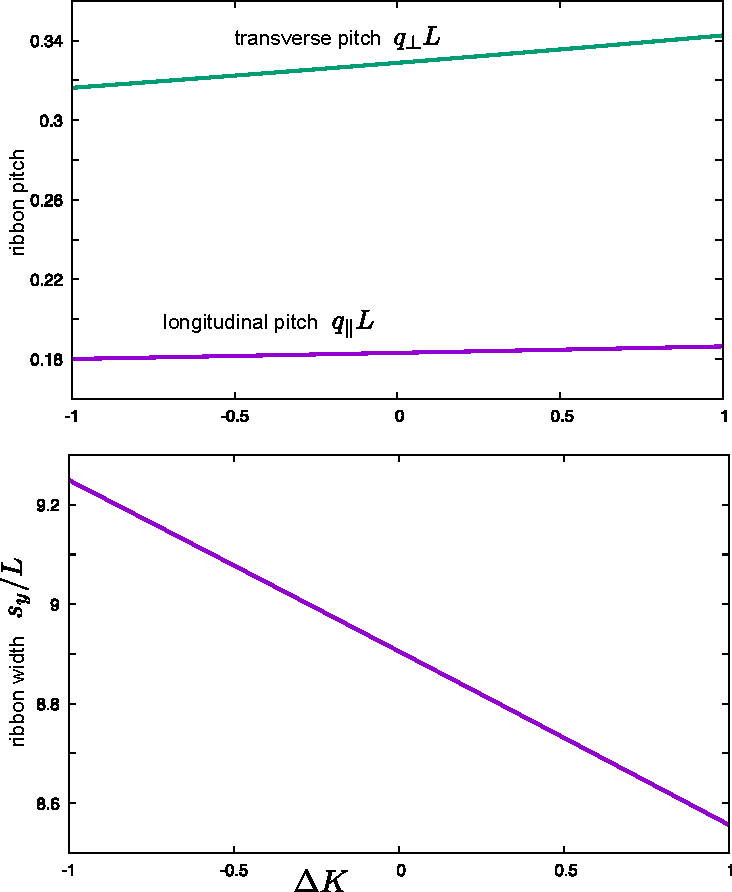
\includegraphics[width=   \columnwidth]{figures/chapter-5/deltak}.
\caption{ \label{ribbontheory} Overview of the ribbon properties as a function of the elastic anisotropy $\Delta K$ [\eq{dk}] of the LC material. Parameters $\lambda_{t} = 0.5 L$ and $q_{0} = 0.4 L^{-1}$. Shown are (a) the longitudinal and transverse ribbon pitches. (b) The equilibrium ribbon width in units rod length $L$. (c) The typical ribbon aspect ratio in terms of the longitudinal pitch versus ribbon width. (d) The tilt angle at the ribbon edge.   }
\end{center}
\end{figure}


Although the expressions obtained are entirely algebraic,  minimization of the total free energy can only be performed numerically. To make progress, we  expand the free energy contributions up to quadratic order in $q$.
Combining terms and reintroducing the twist penetration length $\lambda_{t}$ we arrive at a compact expression for the total free energy per unit length of a weakly twisted ribbon ($q \ll 1/s_{y}$): 
\beq
\frac{F}{K_{2}} \sim   -q q_{0}   +  \frac{1}{2}\left ( \frac{\Delta K}{2} + \frac{L^{2}}{8\lambda_{t}^{2}}\right )  q^{2} + \frac{2 L }{\pi \lambda_{t}^{2}}
\label{flowq}
\eeq
The first two term encodes the free energy change due to (chiral) twist, the second  the effect of splay, bend and saddle-splay elasticity along with depletion, whereas the last term denotes the line tension which up to leading order does not depend on the pitch.  The constant $\Delta K$ represents a combination of the  bend-twist and saddle-twist elastic anisotropies:
\beq
\Delta K = \frac{K_{3}}{K_{2}} - \frac{K_{24}}{K_{2}} + 3
\label{dk}
\eeq
The equilibrium ribbon pitch follows from minimizing \eq{flowq} and is related to $q_{0}$ via:
\begin{align}
q & \sim q_{0} \left ( \frac{\Delta K}{2} + \frac{L^{2}}{8\lambda_{t}^{2}}\right )^{-1}  
\end{align}
Inserting this back into the quadratic free energy and reexpressing all variables in bare units we find:
\beq
\frac{F}{K_{2}} \sim -\frac{1}{2} \left ( \frac{\Delta K}{2} + \frac{L^{2}}{8\lambda_{t}^{2}}\right ) (q_{0} s_{y})^{2} + \frac{2 Ls_{y} }{\pi \lambda_{t}^{2}}
\eeq
which combines a bulk term proportional to $s_{y}^{2}$ and a surface contribution  linear in $s_{y}$. Minimization yield for the typical ribbon width:
\beq
s_{y} \sim \frac{2 L }{ \pi \lambda_{t}^{2} q_{0}^{2} } \left ( \frac{\Delta K}{2} + \frac{L^{2}}{8\lambda_{t}^{2}}\right ) 
\eeq
Finally, we deduce  the ribbon pitch versus width:
\beq
\frac{\textrm{ribbon pitch}}{\textrm{ribbon width}} = \frac{2 \pi}{q s_{y}} \sim  \frac{\pi^{2} q_{0} \lambda_{t}^{2} }{L}
\eeq
and the tilt angle at the ribbon edge:
\beq
\Phi(y = s_{y}/2) = \frac{1}{2} q s_{y} \sim \frac{L}{\pi q_{0} \lambda_{t}^{2}}
\eeq
The predictions above should be qualitatively correct and give valuable insight into how the ribbon properties depend on, for instance, the intrinsic chirality and elasticity of the LC material.  A potential caveat of the low-$q$ expansion, however, is that ribbons form at elevated chirality where the ribbon pitch $qL$ is not necessarily a small parameter ($qL \ll 1$). Because deviations from the simple quadratic free energy \eq{flowq} are to be expected, we chose to minimize the free energy numerically which is an easy task given that all free energy contributions  are in  algebraic form.

In doing so, we may also probe a more general scenario where the twist along the principal ribbon directions is {\em anisotropic}. To this end, we characterize  the twist angles  via $\chi = q_{\parallel} z$ and $\Phi = q_{\perp}y$ in terms of a longitudinal and transverse pitch, $q_{\parallel}$ and $q_{\perp}$, respectively. 
 Typical input values  for the case of {\em fd} rods can be obtained by fixing the twist penetration length $\lambda_{t}  = L/2$ \cite{barry_jpcb2009} and taking a typical (cholesteric) pitch $q_{0} = 0.4L^{-1}$. The elastic anisotropy $\Delta K$ is much harder to specify as it depends quite sensitively on the  saddle-splay modulus $K_{24}$ which is unknown for {\em fd} rods. 
The numerical results are shown in \fig{ribbontheory}. The dependence of the quantities on the elastic anisotropy $\Delta K $ is evident but turns out rather weak, indicating that the predictions should be robust against a wide range of elastic properties of the LC material.   We further observe that the twist is indeed considerably anisotropic with the transverse ribbon pitch being larger than  the longitudinal pitch, while both are {\em smaller} than the typical cholesteric pitch $q_{0}$ that quantifies the chiral strength at the rod level. We further infer that the ribbon width is always a few times the rod length, suggesting that ribbons are indeed very slender quasi-1D  objects. The ribbon pitch-to-width ratio is predicted to be about 3, which is in agreement with experimental observations reported in Ref. \cite{Gibaud2012}. A typical value of 5 was quoted in Kaplan {\em et al.} \cite{kaplan2010theory}  for ribbons of {\em fd} rods mixed with non-adsorbing polymer.   Finally, the edge tilt angle is virtually insensitive to $\Delta K$ and is predicted to be about $84 ^\circ$, confirming that the rods make a near  $\pi/2$-twist at the ribbon edge.

The membrane-ribbon transition   could, in principle, be analyzed by comparing the free energies for both twisted morphologies for a given droplet volume. This however is technically very demanding given that the circular symmetry of the membrane, as encoded in the strongly non-linear elastic free energy \eq{fmem},  precludes a tractable analytical solution of the twist angle unlike for the ribbon. Below, we resort to a hand-waving argument as to why a membrane-ribbon transition should or should not take place. 
 
\section{Membrane or ribbon ? }

Having established a minimal theoretical description for the membranes and  ribbons we now wish to explore under which conditions the various droplet morphologies are favored. It is instructive to consider the main energetic effects involved in shaping the droplets, namely a surface energy and a (bulk) chiral energy that is contained in the twisting of the rods within the droplet. The preference for one state or the other can be argued as resulting from a trade-off between these two energies. On the one hand, for any finite membrane volume (or area) flat circular membranes have a minimal surface free energy but are able to accommodate only a limited amount of twist as the result of twist being expelled from the core and confined into a narrow zone of length $\lambda_{t}$ near the membrane edges. Twisted ribbons, in view of their elongated shape, have an unfavorable perimeter-to-area ratio but are much more efficient at accommodating chirality because the twist is {\em uniform} throughout the main section of the object. Using these arguments, a membrane-to-ribbon transition can  be understood as a natural consequence of a controlled experiment in which enforced chirality driven by cooling the system (a mixture of {\em fd} rods with dextran) was found to lead to a simultaneous reduction of the line tension of the membrane \cite{Gibaud2012}.

We now propose a  heuristic argument for the stability of the membrane  by balancing the bulk chiral and interfacial energetic contributions. First, the chiral free energy contained in the twisted rim of the membrane can be estimated from: 
\beq
\frac{F_{\rm chiral}}{K_{2}} \sim 2 \pi \int_{R_{m} - \lambda_{t}}^{R_{m}} d R R \left [ (\partial_{R} \varphi(R))^{2} + q_{0} \partial_{R} \varphi (R) \right ] 
\eeq
ignoring the depletion and curvature contributions for large membranes ($R_{m} \rightarrow \infty $).  Minimization of the free energy yields an analytical solution for the twist angle versus radius, namely $\varphi(R) = -\frac{q_{0}}{2}R + C_{1} \ln R + C_{2}$. The constants $C_{1}$ and $C_{2}$ can be specified from the following boundary conditions:
\begin{align}
\varphi(R_{m} - \lambda_{t}) &= 0 \nonumber \\ 
\lambda_{t} ^{2}\partial_{R} \varphi(R_{m}) &= \frac{L}{2} \sin \varphi(R_{m}) 
\label{bc}
\end{align}
The first refers to the untwisted core at $R < R_{m} - \lambda_{t}$ while the second follows from the interfacial tension at the membrane edge at $R = R_{m}$.  To simplify matters further we fix the twist penetration length at half the rod length $\lambda_{t} =L/2$ \cite{barry_jpcb2009} and linearize the boundary condition via $ \sin \varphi(R_{m})  \approx \varphi(R_{m}) $. The chiral free energy stored in the membrane rim then reads: 
\beq
\frac{F_{\rm  chiral}}{K_{2}} \sim \frac{\pi}{16} (q_{0}L)^{2} \left ( 1 - \frac{4 R_{m}}{L} \right ) 
\eeq
which is negative for large membranes. This free energy must be balanced against the interfacial contribution which in our minimalist approach reads:
\beq
\frac{F_{\rm  interface}}{K_{2}} \sim \frac{4 \pi R_{m}}{L} \cos \varphi(R_{m})
\eeq
with the edge tilt angle being proportional to the chiral strength via $\varphi(R_{m}) = q_{0}/4$. Equating the two expressions and taking an infinitely large membrane $R_{m} \rightarrow \infty$ we find a critical pitch of $q_{0}^{\ast} L = 3.296$.  This means that below this value the interfacial energy outweighs the gain in chiral energy ($F_{\rm interface} + F_{\rm chiral} >0$) and the membrane is stable. At strong chirality, $q_{0} > q_{0}^{\ast}$ the rim contribution dominates and transitions towards elongated twisted structures such as the ribbon can be expected.  The critical pitch increases for finite-sized membranes given that smaller membranes have a relatively larger rim to surface proportion. The membrane-ribbon transition line based on the non-linearized boundary condition \eq{bc} is easily obtained numerically and is given by the purple curve in \fig{emergent}.  We remark that quantitative predictions from the current expressions have to be taken with care because of our simplistic description of the membrane surface tension which does not account for the effect of chirality and does not include curvature corrections that will play a more prominent for small droplets \cite{malijevsky2012perspective}.  A more general expression for the surface tension $\sigma$ of the droplet should therefore read:
\beq
\sigma(R_{m}) \sim 2 n_{p} a k_{B}T \left ( 1 - \frac{2\delta}{R_{m}} \right ) + \sigma_{\rm chiral}  
\eeq
in terms of the Tolman length $\delta$, which could be positive or negative, and a chirality-dependent correction as conjectured in Ref. \cite{Gibaud2012} for the case of {\em fd}. However, both contributions are unknown for our particular simulation model. It is probable that the chirality contribution is very distinct from the one proposed for the experimental case such that the surface tension is little sensitive or even  decreases with  chirality.  Also, the Tolman length could be negative resulting in $\sigma$ rising  for smaller membrane radii \cite{lei2005tolman,malijevsky2012perspective}.   We may therefore assert that the  small membranes simulated in our study are likely to experience a considerable surface tension that constrains the droplets to remain more or less circular. An alternative strategy to cope with high levels of chirality is then to increase the perimeter of twisted zones at the interior of the membranes by splitting into multiple cores with shared interfaces, reminiscent of domains walls.  Within the interfacial zones between the cores the rods display a $\pi/2$ twist from the local core (see \fig{multidomain}). This enables adjacent cores to share an interface with no incommensurability in the edge twist. The interfacial cost imparted by  the domain walls is likely to be much smaller than that of the membrane and its surrounding polymer fluid.  


\begin{figure}
\begin{center}
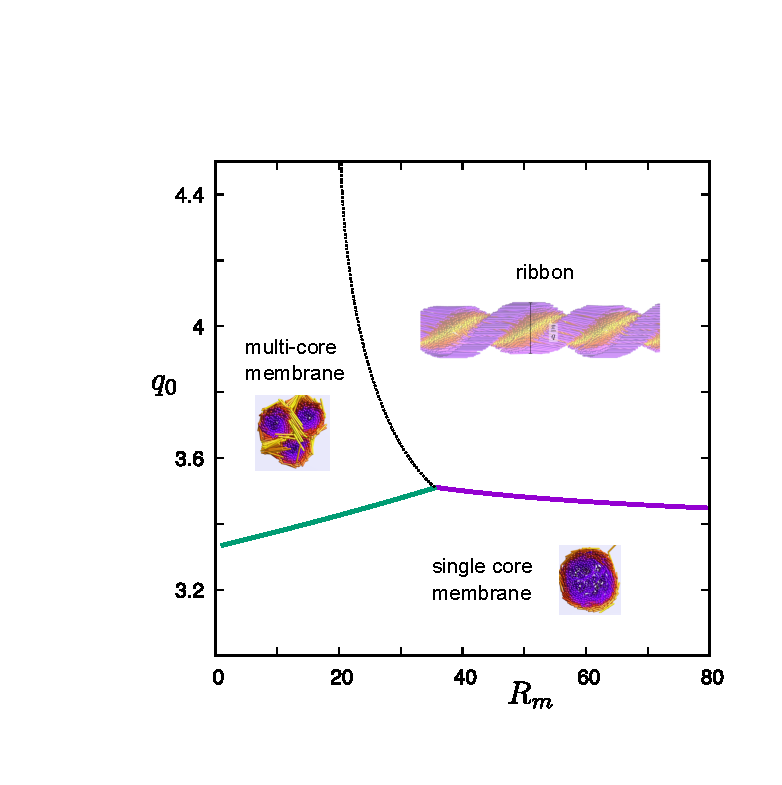
\includegraphics[width=  0.8 \columnwidth]{figures/chapter-5/emergent}.
\caption{ \label{emergent} Overview of the various membrane morphologies predicted for chiral colloidal rods mixed with non-adsorbing polymer as a function of the membrane radius $R_{m}$  and pitch $q_{0}$ (both expressed in units of the rod length $L$). Depending on the membrane radius,  weakly chiral rods tend to self-assemble into single-core twisted membranes but may transition into elongated twisted ribbons beyond a critical chiral strength. Small droplets tend to be curbed by surface tension and are precluded from forming ribbons,  developing into multi-core membranes instead (see also \fig{multidomain}).   }
\end{center}
\end{figure}


 A naive estimate of the transition from the single to a multi-core membrane can be established by comparing the chiral energy of the two states. Let us focus on the simplest case, namely the one composed of three cores [\fig{multidomain}(b) for $\varepsilon_{c}=12$] and denote the radius of each core by $R_{s} = R_{m}/\sqrt{3}$ which guarantees conservation of the total membrane area. Furthermore, we assume that the twist angle at the subcore edge is $\pi/2$ so that the second boundary condition in \eq{bc} should be replaced by $\varphi(R_{s}) = \pi/2 $. Then, the chiral energy contained in each subcore rim reads:
 \beq
 \frac{F_{\rm  chiral}^{(s)}}{K_{2}}  \sim \frac{\pi}{4} q_{0}^{2} \left ( \lambda_{t}^{2} - 2 \lambda_{t} R_{s} \right ) + 2(\pi + \lambda_{t} q_{0} )^{2} \ln \left ( \frac{R_{s} - \lambda_{t}}{R_{s}} \right ) 
 \eeq
Balancing this against the single-core free energy $F_{\rm chiral} = 3 F_{\rm chiral}^{(s)}$ and assuming the interfacial contribution to be the same for both states we find a simple criterion for the onset of multi-domain order. The result is given by the green curve in \fig{emergent}.  In our simulations, we find the single-to-triple core transition to occur around $\varepsilon_{c} =12$.  According to \eq{qzero} for $\rho_{0} \sim 0.5D^{-2}$ this  corresponds to about $q_{0} \approx 0.9$ which is considerably smaller than the value predicted from our naive free energy balance. Combined with the prediction for the (single core) membrane-ribbon transition we construct a tentative state diagram stipulating the conditions for the different morphologies as shown in \fig{emergent}. We speculate that the multi-domain structures, in view of their enhanced capacity to harbour strong twists,  retain their morphology and do not transition into ribbons even at elevated chiral strength. This is tentatively indicates by the dotted black curve. The key conclusion to be drawn  from the diagram is that ribbons are more likely to appear from large membranes (say $R_{m}  > 50 L$) than from small ones. Taking a typical membrane density of $0.5 D^{-2}$ [cf. \fig{density}] we find that the required system size far exceeds the ones probed in our study,  $N > 25 \pi (L/D)^{2} \sim 8000$ for $L/D = 10$.  This clearly poses a significant challenge for future simulation efforts that should be directed towards modelling rod-polymer mixtures using high-performance Molecular Dynamics computations capable of handling system sizes of about an order of magnitude larger than ours. 






%where  $q \ll q_{0}$ depending on the elastic anisotropy and twist penetration length. We remark that the ribbon pitch does not depend on the line tension (second term in \eq{flowq} which is independent of $q$).  

% Check minimize free energy per pitch versus per unit length = 2pi/qq. Combined minimization wrt qq and sy by reverting free energy to bare units rod length.



%Before proceeding with our analysis we immediately infer a couple of basic facts from inspecting \eq{fribbon}. First, as expected chiral forces between the rods, represented by the term proportional to $2-\tau^{2}$, lower the free energy provided the ribbons are sufficiently elongated ($\tau  >\sqrt{2})$. A further stabilization mechanism occurs through the line tension since the curvature correction $w_{2}$ is negative. 

%The relevant constants $\Delta K$ and $\Delta \ell$ can be estimated from the twist penetration length. Taking the reference value $\lambda_{t} = L/2$ quoted for {\em fd} virus rods we find that  $\Delta K \sim (L/2\lambda_{t})^{2} \sim 1 $,  ignoring weak contributions from the bend-to-twist and saddle-splay elasticity. Similarly, we obtain $\Delta \ell \approx 4 $ for a ribbon with a lateral width equal to the rod length $s_{y} = L$. For the pitch we roughly estimate $q_{0} = 2 \pi s_{y} / p_{c} \approx 0.2$ taking a cholesteric pitch  $p_{c} \sim 30L$. 

%The next step is to minimize the free energy \eq{fribbon} with respect to the ribbon pitch $q$ and aspect ratio $\tau$, i.e., $\partial F/\partial q =0$ and $\partial F/\partial \tau =0$ for a given ribbon area $A$. If the line tension is ignored ($\Delta \ell =0$), the extremum condition can be solved analytically and gives an equilibrium ribbon pitch:
%\beq
%q =  \frac{3q_{0}}{4 \Delta K} \frac{(\tau^{2} -2)}{1 + \tau^{2}}
%\eeq
%where the last contribution is a monotonically increasing function for $\tau^{2} >2$ levelling off to unity for $\tau \gg 1$. The ribbon free energy per unit area corresponding to the optimal pitch is:
%\beq
%\frac{F/\tau}{K_{2}}  = -\frac{1}{96} q_{0}  (\tau^{2} -2) q^{3}
%\eeq
%From this we infer that (i) stable ribbons that are not curbed by line tension penalty tend to stretch to very large aspect ratios, and (ii) the limiting pitch at large ribbon aspect ratio is likely smaller than the membrane pitch $q_{0}$ given that $q =  3q_{0}/4 \Delta K$ for $\tau \rightarrow \infty $ and $\Delta K \sim 1$. In practice, conservation of area precludes the ribbons to stretch to infinity while a finite line tension puts a further natural bound to $\tau$. 



%\subsection{Effect of anisotropic twist} 

%\begin{figure}
%\begin{center}
%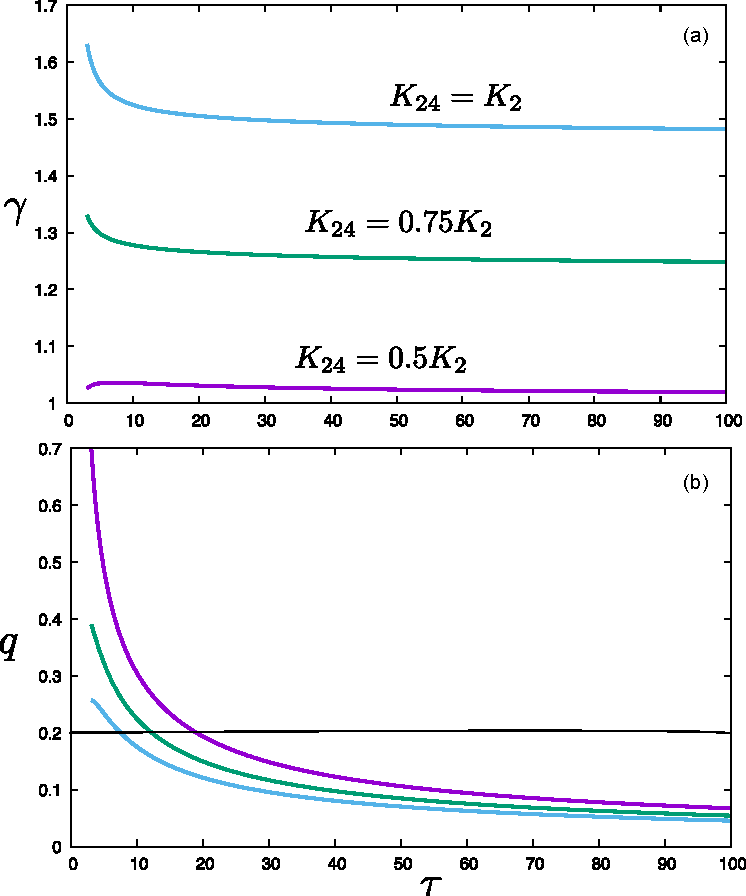
\includegraphics[width=  0.5 \columnwidth]{figures/chapter-5/raniso}.
%\caption{ \label{fig3} Twist anisotropy $\gamma$ and pitch $q$ of a twisted ribbon with width $s_{y} = L$ as a function of the %ribbon length $\tau$. The chiral strength between the rods is given by the membrane pitch $q_{0} = 0.2L^{-1}$ (horizontal black %line). The twist penetration length is $\lambda_{t} = 0.5L $.   }
%\end{center}
%\end{figure}


%Let us now explore the possibility of unequal twist along the short and long ribbon axes. This should render a more realistic picture of the internal twist profile of the ribbon  given that the twist along the principal ribbon directions need not have the same magnitude. We proceed by allowing $\gamma$, which denotes the ratio between the degree of twist along the long and short axes  of the ribbon,  to be a  variable quantity. Working out the algebraic free energy per area we find for the bulk elastic contribution:
%\begin{align}
%\frac{F}{ K_{2} \tau} &\sim 
%\frac{1}{24} \left [ \frac{K_{3}}{K_{2}} q^{4} (1 + \tau^{2}) \gamma^{2} + B\right ]
%\end{align}
%with $B$ the twist elastic contribution:
%\beq
%B = (q_{0} + q - q \gamma) (12 q_{0} + q (12 - \gamma (12 + q^2 ( \tau^{2} \gamma -2))))
%\eeq
%This term reduces to the much simpler expression explored in the previous section for the isotropic twist case ($\gamma =1$). Similarly, the saddle-splay term now becomes:
%\beq
% \frac{F}{K_{2} \tau} \sim  - \frac{1}{24}\frac{K_{24}}{ K_{2} } q^{4} \gamma (1 + \tau^{2} \gamma)
%\eeq
%Finally the depletion free energy reads (ignoring irrelevant constants as well as the line tension contribution):
%\beq
% \frac{F}{K_{2} \tau} \sim  \frac{L^{2}}{96 \lambda_{t}^{2}} q^{4} (1 + \tau^{2} \gamma^{4})
%\eeq
%Clearly, these complex expressions are no longer amenable to further analytical treatment. Furthermore, the elastic and depletion strengths can longer be compactly combined into a  single parameter $\eq{dk}$ as could be done for the isotropic twist case but must be  separately defined. However, minimization of the three free energy terms above with respect to $q$ and $\gamma$ is easily carried out numerically and the results are shown in \fig{fig3} taking $K_{3}/K_{2} = 1/4$, $q_{0} = 0.2$, $\lambda_{t} = L/2$ and three different values for the saddle-splay elastic modulus. Clearly,  $\gamma $ tends to be larger than unity depending on the strength of the saddle-splay elasticity $K_{24}$ indicating twisting along the main ribbon axis can be about 30-50 \% stronger than across the short axis. We remark that $K_{24}$ plays an essential role in driving the  twist for the ribbon geometry. In fact, saddle-splay elasticity cannot be ignored given that  no physical solutions of the minimization problem were found  for $K_{24} =0$. The lowest value explored ($K_{24} = K_{2}/2$) roughly recovers the previous scenario of equal twist along the short and long ribbon axes. The fact that a positive value of the $K_{24}$ is required for stabilizing ribbons is consistent with the work of Kaplan {\rm et al.} \cite{kaplan2010theory} providing a more wide-ranging theoretical framework for membranes and ribbons  based on a Helfrich-DeGennes model which also considers the effect of layer bending (ignored in our model).  

%We further conclude from \fig{fig3}b that longer ribbons tend to be less twisted than short ones.   Short ribbons ($\tau <10$) seem {\em overtwisted} compared to that of the equivalent (single twist) cholesteric phase while long ribbons experience less twist. In all cases we see that $q$ levels off to a limiting value $q < q_{0}$ for infinitely stretched ribbons ($\tau \rightarrow \infty$) in line with our analytical predictions for the case of constrained isotropic twist $\gamma =1$. The line tension, ignored in the results of \fig{fig3}, will put a constraint on the optimal aspect ratio $\tau$ which needs to optimized along with $q$ and $\gamma$ for a given ribbon area. We will not pursue this further in this study given that, in experiment, the line tension at the starfish transition is very low while the available virus material and hence the area tends to be quite large. Both  factors enable these ribbons to grow into strongly elongated objects. This should be compared to our predictions for the limiting case $\tau \rightarrow \infty$. Further restriction  to applying our model to experiments relates to the unknown saddle-splay constant for {\em fd} virus rods. 

%A further characteristic we may deduce from our model is the typical long-axis pitch, in the experiments simply referred to as the pitch,  versus ribbon width.  This ratio of length scales is given by:
%\beq
%\frac{\textrm{ribbon   pitch}}{\textrm{ribbon width}} \sim \frac{2 \pi}{\gamma q s_{y}} 
%\eeq
%From the optical microscopy pictures provided in Ref.  \cite{Gibaud2012} we roughly infer that this ratio should be about 2-3. Taking ribbons of moderate length, say  $\tau = 5$, we find that the predicted ratio is somewhat larger ($\sim 10$), in qualitative agreement with experimental observation.




\section{Conclusions}

%Inspired by recent experimental observations of nmorphological transition of LC membranes colloidal rods mixed with non-adsorbing polymers we have embarked on   Using large scale Monte Carlo simulations combined with liquid crystal continuum theory based onthe Frank elasticity  we have explored mesoscale droplet of colloirdal rods mixed with non-adsorbing polymer



\clearpage








